\section{Xây dựng Use Case Diagram}
\subsection{Use case Diagram tổng quát}
\begin{figure}[H]
    \centering
    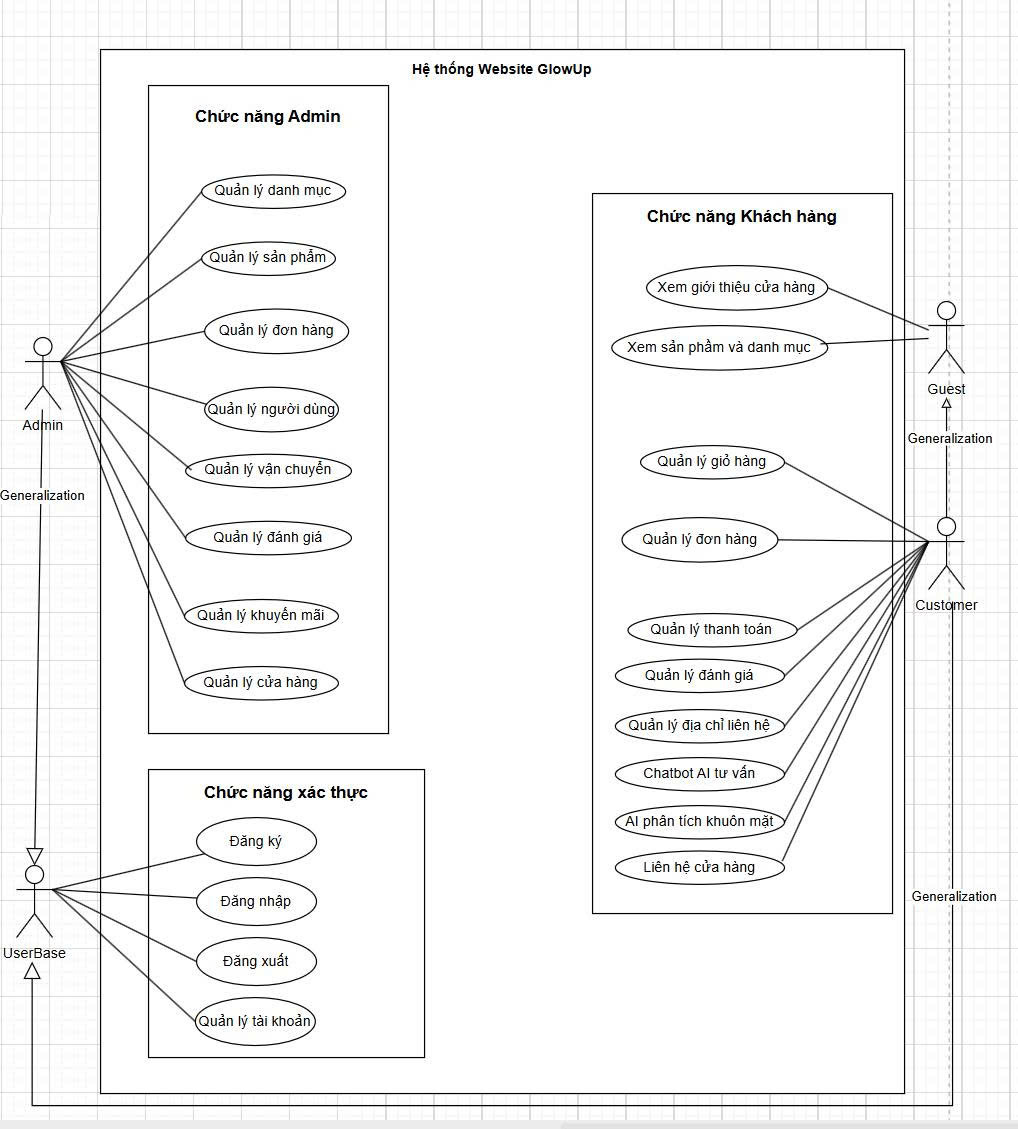
\includegraphics[scale=0.3]{graphics/main/chapter2/section2/usecasetq.jpg}
    \caption{Use case Diagram tổng quát}
    \label{fig:usecase_overall}
\end{figure}
Các Actor trong hệ thống bao gồm:
\begin{itemize}[noitemsep]
    \item \textbf{UserBase}: 
    Là actor cơ sở đại diện cho tất cả người dùng của hệ thống. UserBase thực hiện các chức năng xác thực và quản lý tài khoản bao gồm: đăng ký, đăng nhập, đăng xuất, đăng nhập qua Google OAuth và quản lý hồ sơ cá nhân.

    \item \textbf{Customer}: 
    Là actor kế thừa từ UserBase, đại diện cho khách hàng đã đăng nhập hệ thống. Customer có thể thực hiện đầy đủ các chức năng: xem giới thiệu cửa hàng, xem sản phẩm và danh mục, quản lý giỏ hàng, quản lý đơn hàng, quản lý thanh toán qua Stripe, quản lý đánh giá sản phẩm, quản lý địa chỉ liên hệ, theo dõi đơn hàng, sử dụng Chat AI tư vấn, thử đồ ảo qua FitDit AI, thử đồ qua Snap Camera và nhận gợi ý size phù hợp.

    \item \textbf{Guest}: 
    Là actor kế thừa từ Customer, đại diện cho người dùng chưa đăng nhập. Guest chỉ có thể thực hiện các chức năng cơ bản như: xem giới thiệu cửa hàng và xem sản phẩm cùng danh mục.

    \item \textbf{Admin}: 
    Là actor kế thừa từ UserBase, đại diện cho quản trị viên hệ thống. Admin thực hiện các chức năng quản trị bao gồm: quản lý danh mục, quản lý sản phẩm, quản lý đơn hàng, quản lý người dùng, quản lý vận chuyển, quản lý đánh giá, quản lý AI/AR, quản lý voucher, quản lý cửa hàng và thống kê doanh thu.
\end{itemize}

% ================================================================
\subsection{Use case Diagram chức năng xác thực}
\begin{figure}[H]
    \centering
    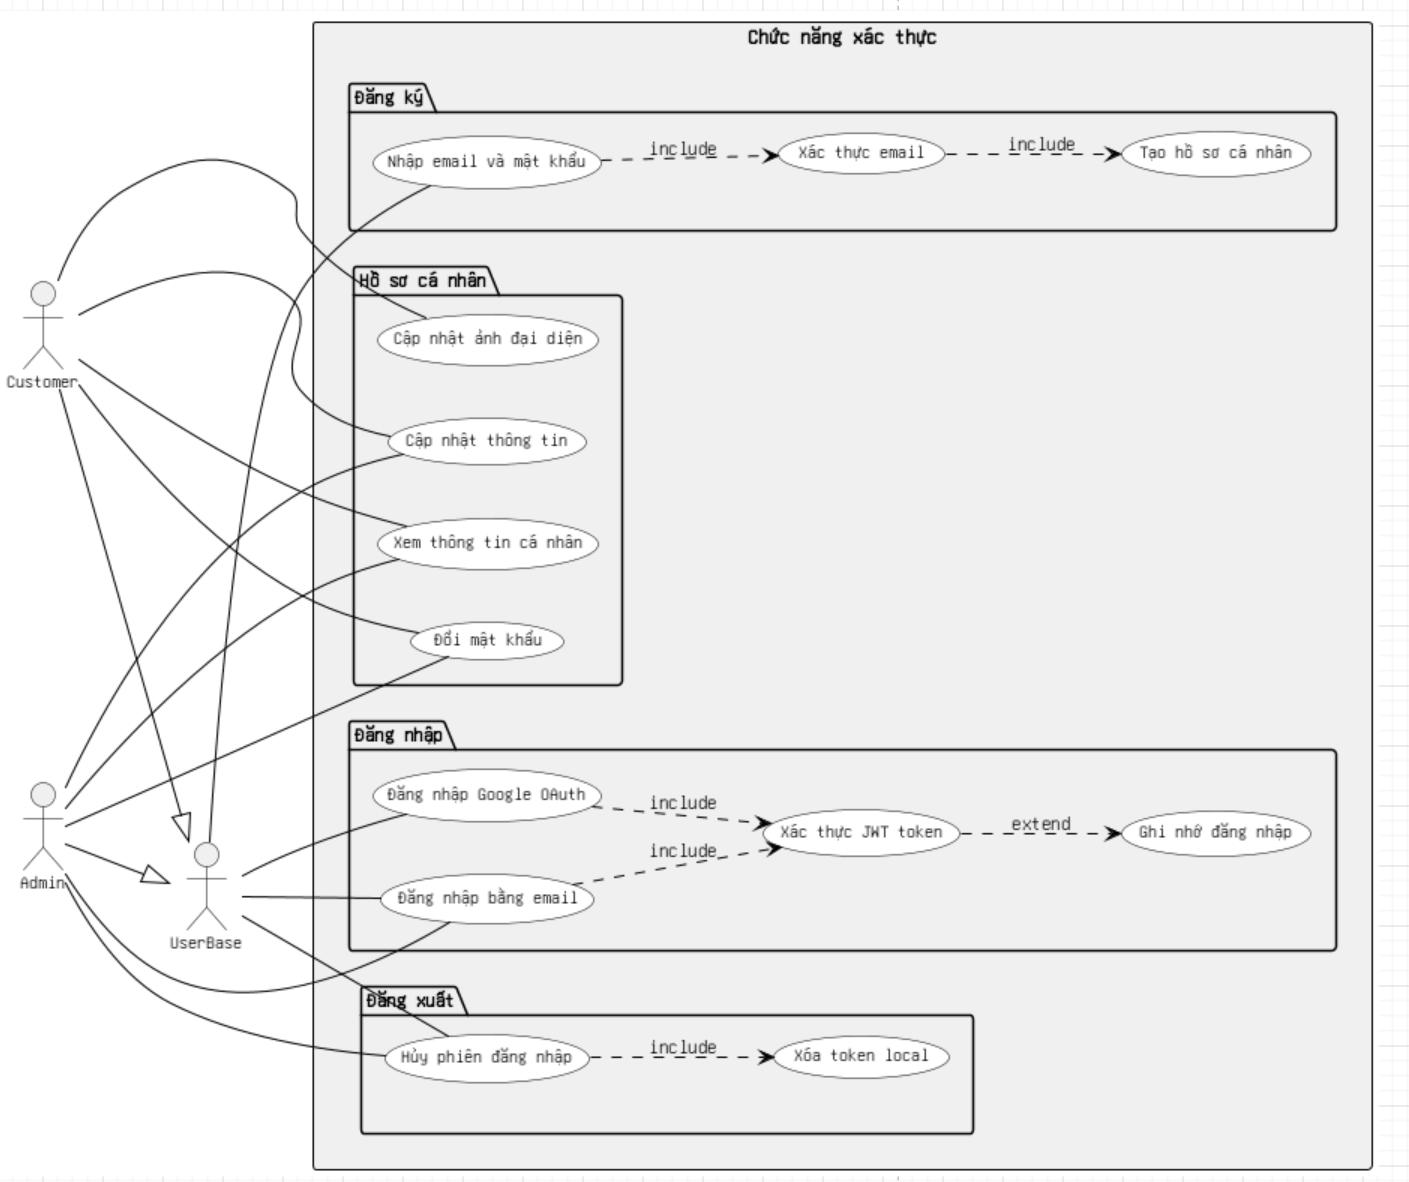
\includegraphics[width=0.8\textwidth]{graphics/main/chapter2/section2/uc_auth.jpg}
    \caption{Use case Diagram chức năng xác thực}
    \label{fig:usecase_auth}
\end{figure}

\subsubsection{Đặc tả use case chức năng xác thực}

\begin{table}[H]
\centering
\caption{Đặc tả use case: Đăng ký}
\begin{tabularx}{\textwidth}{|l|X|}
\hline
\textbf{Tên use case} & Đăng ký \\
\hline
\textbf{Actor} & UserBase \\
\hline
\textbf{Mô tả} & Người dùng tạo tài khoản mới bằng email và mật khẩu. \\
\hline
\textbf{Tiền điều kiện} & Người dùng chưa có tài khoản. \\
\hline
\textbf{Luồng chính} &
\begin{enumerate}[noitemsep,topsep=0pt]
    \item Người dùng nhập email và mật khẩu.
    \item Hệ thống gửi email xác thực \textit{«include»}.
    \item Người dùng xác nhận email.
    \item Hệ thống tạo hồ sơ cá nhân \textit{«include»}.
\end{enumerate} \\
\hline
\textbf{Hậu điều kiện} & Tài khoản được tạo, người dùng có thể đăng nhập. \\
\hline
\end{tabularx}
\end{table}

\begin{table}[H]
\centering
\caption{Đặc tả use case: Đăng nhập}
\begin{tabularx}{\textwidth}{|l|X|}
\hline
\textbf{Tên use case} & Đăng nhập \\
\hline
\textbf{Actor} & UserBase (Customer, Admin) \\
\hline
\textbf{Mô tả} & Người dùng xác thực danh tính để truy cập hệ thống. \\
\hline
\textbf{Tiền điều kiện} & Người dùng đã có tài khoản. \\
\hline
\textbf{Luồng chính} &
\begin{enumerate}[noitemsep,topsep=0pt]
    \item Người dùng chọn đăng nhập bằng email hoặc Google OAuth.
    \item Hệ thống xác thực JWT token \textit{«include»}.
    \item Hệ thống tùy chọn ghi nhớ đăng nhập \textit{«extend»}.
    \item Chuyển hướng đến trang tương ứng theo vai trò.
\end{enumerate} \\
\hline
\textbf{Hậu điều kiện} & Phiên đăng nhập được khởi tạo, JWT token được lưu. \\
\hline
\end{tabularx}
\end{table}

\begin{table}[H]
\centering
\caption{Đặc tả use case: Đăng xuất}
\begin{tabularx}{\textwidth}{|l|X|}
\hline
\textbf{Tên use case} & Đăng xuất \\
\hline
\textbf{Actor} & UserBase (Customer, Admin) \\
\hline
\textbf{Mô tả} & Người dùng kết thúc phiên làm việc hiện tại. \\
\hline
\textbf{Tiền điều kiện} & Người dùng đang đăng nhập. \\
\hline
\textbf{Luồng chính} &
\begin{enumerate}[noitemsep,topsep=0pt]
    \item Người dùng chọn đăng xuất.
    \item Hệ thống hủy phiên đăng nhập \textit{«include»}.
    \item Hệ thống xóa token lưu cục bộ \textit{«include»}.
    \item Chuyển hướng về trang đăng nhập.
\end{enumerate} \\
\hline
\textbf{Hậu điều kiện} & Phiên đăng nhập bị hủy, token bị xóa. \\
\hline
\end{tabularx}
\end{table}

\begin{table}[H]
\centering
\caption{Đặc tả use case: Hồ sơ cá nhân}
\begin{tabularx}{\textwidth}{|l|X|}
\hline
\textbf{Tên use case} & Hồ sơ cá nhân \\
\hline
\textbf{Actor} & Customer, Admin \\
\hline
\textbf{Mô tả} & Người dùng xem và cập nhật thông tin tài khoản cá nhân. \\
\hline
\textbf{Tiền điều kiện} & Người dùng đã đăng nhập. \\
\hline
\textbf{Luồng chính} &
\begin{enumerate}[noitemsep,topsep=0pt]
    \item Người dùng truy cập trang hồ sơ.
    \item Hệ thống hiển thị thông tin hiện tại.
    \item Người dùng chỉnh sửa thông tin / đổi mật khẩu / cập nhật ảnh đại diện.
    \item Hệ thống xác nhận và lưu thay đổi.
\end{enumerate} \\
\hline
\textbf{Hậu điều kiện} & Thông tin tài khoản được cập nhật. \\
\hline
\end{tabularx}
\end{table}

% ================================================================
\subsection{Use case Diagram chức năng admin quản lý danh mục sản phẩm}
\begin{figure}[H]
    \centering
    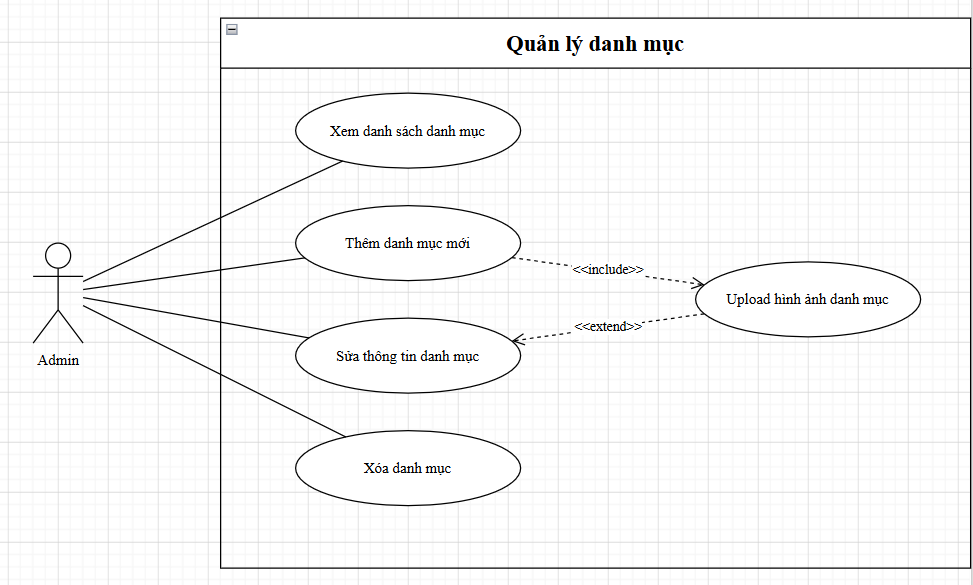
\includegraphics[width=0.8\textwidth]{graphics/main/chapter2/section2/uc_danh_muc.jpg}
    \caption{Use case Diagram chức năng admin quản lý danh mục sản phẩm}
    \label{fig:usecase_danh_muc}
\end{figure}

\subsubsection{Đặc tả use case chức năng admin quản lý danh mục sản phẩm}

\begin{longtable}{|>{\raggedright\arraybackslash}p{2cm}|>{\raggedright\arraybackslash}p{2.5cm}|>{\raggedright\arraybackslash}p{4cm}|>{\raggedright\arraybackslash}p{5.5cm}|}
\caption{Đặc tả use case chức năng admin quản lý danh mục sản phẩm}
\label{tab:uc_admin_category} \\
\hline
\rowcolor{header}\textcolor{white}{\textbf{Mã UC}} & \textcolor{white}{\textbf{Tên}} & \textcolor{white}{\textbf{Luồng chính}} & \textcolor{white}{\textbf{Ngoại lệ / Thay thế}} \\
\hline
\endfirsthead
\caption[]{Đặc tả use case chức năng admin quản lý danh mục sản phẩm (tiếp theo)} \\
\hline
\rowcolor{header}\textcolor{white}{\textbf{Mã UC}} & \textcolor{white}{\textbf{Tên}} & \textcolor{white}{\textbf{Luồng chính}} & \textcolor{white}{\textbf{Ngoại lệ / Thay thế}} \\
\hline
\endhead

UC1 & Xem danh sách danh mục &
  \textbf{Tiền ĐK:} Đã đăng nhập. \newline
  1. Admin truy cập trang quản lý danh mục. \newline
  2. Hệ thống truy vấn và hiển thị danh sách danh mục. &
  Không có danh mục $\to$ hiển thị danh sách trống. \\
\hline

UC2 & Thêm danh mục mới &
  \textbf{Tiền ĐK:} Đã đăng nhập. \newline
  1. Admin nhập tên danh mục. \newline
  2. \textit{[include]} UC5: Upload hình ảnh. \newline
  3. Hệ thống xác thực và lưu vào CSDL. \newline
  \textbf{Hậu ĐK:} Danh mục mới được tạo. &
  Tên đã tồn tại $\to$ thông báo lỗi, yêu cầu nhập lại. \\
\hline

UC3 & Sửa thông tin danh mục &
  \textbf{Tiền ĐK:} Đã đăng nhập; danh mục tồn tại. \newline
  1. Admin chọn danh mục cần sửa. \newline
  2. Chỉnh sửa tên danh mục. \newline
  3. \textit{[extend]} UC5: Upload ảnh mới nếu cần. \newline
  4. Hệ thống xác thực và lưu thay đổi. &
  Tên mới trùng danh mục khác $\to$ thông báo lỗi. \\
\hline

UC4 & Xóa danh mục &
  \textbf{Tiền ĐK:} Đã đăng nhập; danh mục tồn tại. \newline
  1. Admin chọn danh mục cần xóa. \newline
  2. Hệ thống hiển thị hộp thoại xác nhận. \newline
  3. Admin xác nhận $\to$ hệ thống xóa. \newline
  \textbf{Hậu ĐK:} Danh mục bị xóa khỏi CSDL. &
  Hủy thao tác $\to$ không thay đổi. \newline
  Danh mục đang được sử dụng $\to$ không cho phép xóa. \\
\hline

UC5 & Upload hình ảnh danh mục &
  \textbf{Tiền ĐK:} Đang thực hiện UC2 (bắt buộc) hoặc UC3 (tùy chọn). \newline
  1. Admin chọn file ảnh từ thiết bị. \newline
  2. Hệ thống kiểm tra định dạng và kích thước. \newline
  3. Hệ thống lưu ảnh và cập nhật đường dẫn vào danh mục. &
  Sai định dạng $\to$ thông báo lỗi. \newline
  Vượt kích thước giới hạn $\to$ yêu cầu chọn lại. \\
\hline

\end{longtable}

% ================================================================
\subsection{Use case Diagram chức năng admin quản lý sản phẩm}
\begin{figure}[H]
    \centering
    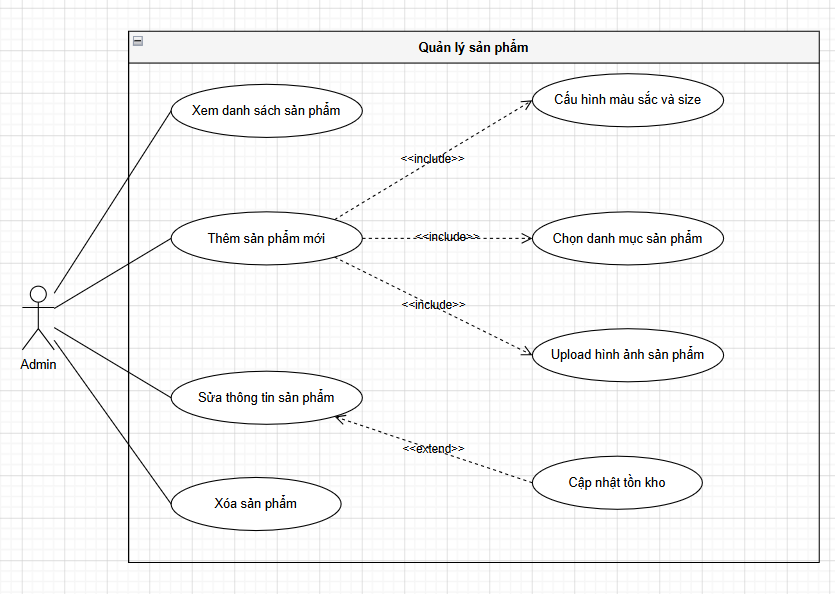
\includegraphics[width=0.8\textwidth]{graphics/main/chapter2/section2/uc_sp.jpg}
    \caption{Use case Diagram chức năng admin quản lý sản phẩm}
    \label{fig:usecase_sp}
\end{figure}

\subsubsection{Đặc tả use case chức năng admin quản lý sản phẩm}

\begin{longtable}{|>{\raggedright\arraybackslash}p{2cm}|>{\raggedright\arraybackslash}p{2.5cm}|>{\raggedright\arraybackslash}p{4cm}|>{\raggedright\arraybackslash}p{5.5cm}|}
\caption{Đặc tả use case chức năng admin quản lý sản phẩm}
\label{tab:uc_admin_product} \\
\hline
\rowcolor{header}\textcolor{white}{\textbf{Mã UC}} & \textcolor{white}{\textbf{Tên}} & \textcolor{white}{\textbf{Luồng chính}} & \textcolor{white}{\textbf{Ngoại lệ / Thay thế}} \\
\hline
\endfirsthead
\caption[]{Đặc tả use case chức năng admin quản lý sản phẩm (tiếp theo)} \\
\hline
\rowcolor{header}\textcolor{white}{\textbf{Mã UC}} & \textcolor{white}{\textbf{Tên}} & \textcolor{white}{\textbf{Luồng chính}} & \textcolor{white}{\textbf{Ngoại lệ / Thay thế}} \\
\hline
\endhead

UC1 & Xem danh sách sản phẩm &
  \textbf{Tiền ĐK:} Đã đăng nhập. \newline
  1. Admin truy cập trang quản lý sản phẩm. \newline
  2. Hệ thống hiển thị danh sách sản phẩm (tên, danh mục, giá, tồn kho, trạng thái). \newline
  3. Admin lọc theo danh mục hoặc tìm kiếm theo tên. &
  Không có sản phẩm phù hợp $\to$ hiển thị danh sách trống. \\
\hline

UC2 & Thêm sản phẩm mới &
  \textbf{Tiền ĐK:} Đã đăng nhập. \newline
  1. Admin nhập tên, mô tả, giá sản phẩm. \newline
  2. \textit{[include]} UC6: Chọn danh mục. \newline
  3. \textit{[include]} UC5: Upload hình ảnh. \newline
  4. \textit{[include]} UC7: Cấu hình màu sắc và size. \newline
  5. Hệ thống xác thực và lưu vào CSDL. \newline
  \textbf{Hậu ĐK:} Sản phẩm mới được tạo. &
  Thiếu trường bắt buộc $\to$ lỗi validation. \newline
  Tên đã tồn tại $\to$ thông báo lỗi, yêu cầu nhập lại. \\
\hline

UC3 & Sửa thông tin sản phẩm &
  \textbf{Tiền ĐK:} Đã đăng nhập; sản phẩm tồn tại. \newline
  1. Admin chọn sản phẩm cần sửa. \newline
  2. Hệ thống hiển thị thông tin hiện tại. \newline
  3. Admin chỉnh sửa các trường cần thay đổi. \newline
  4. \textit{[extend]} UC8: Cập nhật tồn kho nếu cần. \newline
  5. Hệ thống xác thực và lưu thay đổi. &
  Tên mới trùng sản phẩm khác $\to$ thông báo lỗi. \newline
  Lỗi lưu dữ liệu $\to$ không thay đổi sản phẩm. \\
\hline

UC4 & Xóa sản phẩm &
  \textbf{Tiền ĐK:} Đã đăng nhập; sản phẩm tồn tại. \newline
  1. Admin chọn sản phẩm cần xóa. \newline
  2. Hệ thống hiển thị hộp thoại xác nhận. \newline
  3. Admin xác nhận $\to$ hệ thống xóa sản phẩm và các biến thể liên quan. \newline
  \textbf{Hậu ĐK:} Sản phẩm bị xóa khỏi CSDL. &
  Hủy thao tác $\to$ không thay đổi. \newline
  Sản phẩm đang có trong đơn hàng chưa hoàn tất $\to$ không cho phép xóa. \\
\hline

UC5 & Upload hình ảnh sản phẩm &
  \textbf{Tiền ĐK:} Đang thực hiện UC2 hoặc UC3. \newline
  1. Admin chọn file ảnh từ thiết bị. \newline
  2. Hệ thống kiểm tra định dạng và kích thước. \newline
  3. Hệ thống lưu ảnh và cập nhật đường dẫn vào sản phẩm. &
  Sai định dạng $\to$ thông báo lỗi. \newline
  Vượt kích thước giới hạn $\to$ yêu cầu chọn lại. \\
\hline

UC6 & Chọn danh mục sản phẩm &
  \textbf{Tiền ĐK:} Đang thực hiện UC2; ít nhất một danh mục tồn tại. \newline
  1. Hệ thống hiển thị danh sách danh mục hiện có. \newline
  2. Admin chọn danh mục phù hợp cho sản phẩm. \newline
  3. Hệ thống ghi nhận danh mục đã chọn. &
  Chưa có danh mục nào $\to$ yêu cầu tạo danh mục trước. \\
\hline

UC7 & Cấu hình màu sắc và size &
  \textbf{Tiền ĐK:} Đang thực hiện UC2. \newline
  1. Admin thêm các biến thể (màu sắc, size). \newline
  2. Admin nhập số lượng tồn kho và giá cho từng biến thể. \newline
  3. Hệ thống lưu danh sách biến thể vào sản phẩm. \newline
  \textbf{Hậu ĐK:} Biến thể sản phẩm được tạo trong CSDL. &
  Số lượng tồn kho nhập âm $\to$ lỗi validation. \newline
  Chưa thêm biến thể nào $\to$ cảnh báo trước khi lưu. \\
\hline

UC8 & Cập nhật tồn kho &
  \textbf{Tiền ĐK:} Đang thực hiện UC3; biến thể sản phẩm tồn tại. \newline
  1. Admin chọn biến thể cần cập nhật tồn kho. \newline
  2. Admin nhập số lượng mới. \newline
  3. Hệ thống lưu thay đổi vào CSDL. \newline
  \textbf{Hậu ĐK:} Tồn kho được cập nhật. &
  Số lượng nhập âm $\to$ lỗi validation. \\
\hline

\end{longtable}

% ================================================================
\subsection{Use case Diagram chức năng admin quản lý đơn hàng}
\begin{figure}[H]
    \centering
    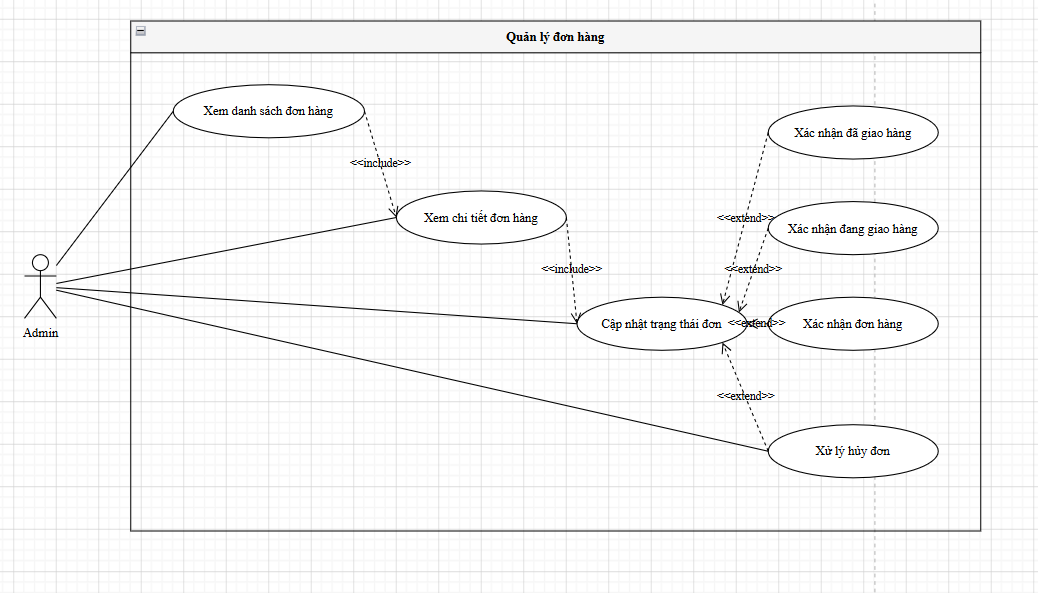
\includegraphics[width=0.8\textwidth]{graphics/main/chapter2/section2/uc_don_hang.jpg}
    \caption{Use case Diagram chức năng admin quản lý đơn hàng}
    \label{fig:usecase_don_hang}
\end{figure}

\subsubsection{Đặc tả use case chức năng admin quản lý đơn hàng}

\begin{longtable}{|>{\raggedright\arraybackslash}p{2cm}|>{\raggedright\arraybackslash}p{2.5cm}|>{\raggedright\arraybackslash}p{4cm}|>{\raggedright\arraybackslash}p{5.5cm}|}
\caption{Đặc tả use case chức năng admin quản lý đơn hàng}
\label{tab:uc_admin_order} \\
\hline
\rowcolor{header}\textcolor{white}{\textbf{Mã UC}} & \textcolor{white}{\textbf{Tên}} & \textcolor{white}{\textbf{Luồng chính}} & \textcolor{white}{\textbf{Ngoại lệ / Thay thế}} \\
\hline
\endfirsthead
\caption[]{Đặc tả use case chức năng admin quản lý đơn hàng (tiếp theo)} \\
\hline
\rowcolor{header}\textcolor{white}{\textbf{Mã UC}} & \textcolor{white}{\textbf{Tên}} & \textcolor{white}{\textbf{Luồng chính}} & \textcolor{white}{\textbf{Ngoại lệ / Thay thế}} \\
\hline
\endhead

UC1 & Xem danh sách đơn hàng &
  \textbf{Tiền ĐK:} Đã đăng nhập. \newline
  1. Admin truy cập trang quản lý đơn hàng. \newline
  2. Hệ thống hiển thị danh sách đơn hàng (mã đơn, khách hàng, ngày đặt, trạng thái, tổng tiền). \newline
  3. Admin lọc theo trạng thái hoặc tìm kiếm theo mã đơn. \newline
  4. \textit{[include]} UC2: Xem chi tiết khi chọn đơn. &
  Không có đơn phù hợp $\to$ hiển thị danh sách trống. \newline
  Lỗi CSDL $\to$ thông báo lỗi, yêu cầu thử lại. \\
\hline

UC2 & Xem chi tiết đơn hàng &
  \textbf{Tiền ĐK:} Đã chọn đơn hàng từ UC1. \newline
  1. Hệ thống hiển thị: sản phẩm, thông tin khách, địa chỉ giao, phương thức thanh toán, lịch sử trạng thái. \newline
  2. \textit{[include]} UC3: Hiển thị hành động theo trạng thái hiện tại. &
  Đơn không tồn tại $\to$ thông báo lỗi, quay về danh sách. \\
\hline

UC3 & Cập nhật trạng thái đơn &
  \textbf{Tiền ĐK:} Đang xem UC2; đơn ở trạng thái cho phép chuyển đổi. \newline
  1. Admin chọn trạng thái mục tiêu (kích hoạt UC4/UC5/UC6/UC7). \newline
  2. Hệ thống yêu cầu xác nhận. \newline
  3. Admin xác nhận $\to$ hệ thống lưu, ghi lịch sử, gửi thông báo khách. \newline
  \textbf{Hậu ĐK:} Trạng thái đơn được cập nhật. &
  Admin hủy $\to$ giữ nguyên trạng thái cũ. \newline
  Lỗi lưu dữ liệu $\to$ không thay đổi trạng thái. \\
\hline

UC4 & Xác nhận đơn hàng &
  \textbf{Tiền ĐK:} Đơn ở trạng thái \textit{chờ xác nhận}. \newline
  1. Admin kiểm tra tồn kho và xác nhận đơn. \newline
  2. Hệ thống chuyển trạng thái sang \textit{đã xác nhận} và thông báo khách. \newline
  \textbf{Hậu ĐK:} Đơn chuyển sang \textit{đã xác nhận}. &
  Sản phẩm hết hàng $\to$ chuyển sang UC7. \\
\hline

UC5 & Xác nhận đang giao hàng &
  \textbf{Tiền ĐK:} Đơn ở trạng thái \textit{đã xác nhận}. \newline
  1. Admin xác nhận đơn đã bàn giao cho đơn vị vận chuyển. \newline
  2. Hệ thống chuyển trạng thái, ghi thời điểm bắt đầu giao và thông báo khách. \newline
  \textbf{Hậu ĐK:} Đơn chuyển sang \textit{đang giao hàng}. &
  Không có. \\
\hline

UC6 & Xác nhận đã giao hàng &
  \textbf{Tiền ĐK:} Đơn ở trạng thái \textit{đang giao hàng}. \newline
  1. Admin nhận xác nhận giao thành công. \newline
  2. Hệ thống chuyển trạng thái, ghi thời điểm hoàn tất và thông báo khách. \newline
  \textbf{Hậu ĐK:} Đơn chuyển sang \textit{đã giao hàng}. &
  Giao thất bại $\to$ Admin quyết định giao lại hoặc chuyển UC7. \\
\hline

UC7 & Xử lý hủy đơn &
  \textbf{Tiền ĐK:} Đơn chưa ở trạng thái \textit{đã giao hàng}. \newline
  1. Admin nhận yêu cầu hủy, kiểm tra lý do và trạng thái thanh toán. \newline
  2. Admin nhập lý do hủy và xác nhận. \newline
  3. Hệ thống cập nhật trạng thái, hoàn tồn kho, khởi tạo hoàn tiền (nếu đã thanh toán) và thông báo khách. \newline
  \textbf{Hậu ĐK:} Đơn chuyển sang \textit{đã hủy}. &
  Từ chối hủy (đơn đang giao) $\to$ thông báo từ chối đến khách. \newline
  Lỗi hoàn tiền $\to$ ghi log, xử lý thủ công. \\
\hline

\end{longtable}
% ================================================================
\subsection{Use case Diagram chức năng admin quản lý người dùng}
\begin{figure}[H]
    \centering
    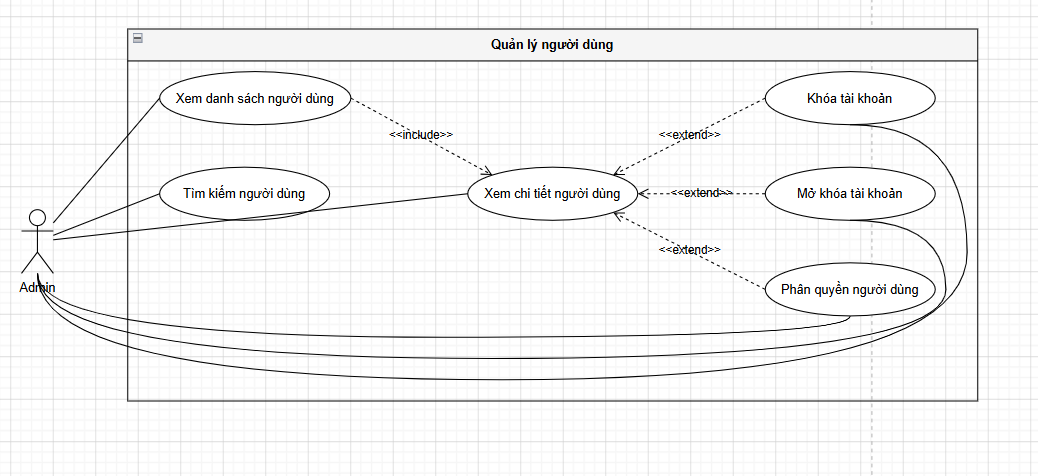
\includegraphics[width=0.8\textwidth]{graphics/main/chapter2/section2/uc_user.jpg}
    \caption{Use case Diagram chức năng admin quản lý người dùng}
    \label{fig:usecase_user}
\end{figure}

\subsubsection{Đặc tả use case chức năng admin quản lý người dùng}

\begin{longtable}{|>{\raggedright\arraybackslash}p{2cm}|>{\raggedright\arraybackslash}p{2.5cm}|>{\raggedright\arraybackslash}p{4cm}|>{\raggedright\arraybackslash}p{5.5cm}|}
\caption{Đặc tả use case chức năng admin quản lý người dùng}
\label{tab:uc_admin_user} \\
\hline
\rowcolor{header}\textcolor{white}{\textbf{Mã UC}} & \textcolor{white}{\textbf{Tên}} & \textcolor{white}{\textbf{Luồng chính}} & \textcolor{white}{\textbf{Ngoại lệ / Thay thế}} \\
\hline
\endfirsthead
\caption[]{Đặc tả use case chức năng admin quản lý người dùng (tiếp theo)} \\
\hline
\rowcolor{header}\textcolor{white}{\textbf{Mã UC}} & \textcolor{white}{\textbf{Tên}} & \textcolor{white}{\textbf{Luồng chính}} & \textcolor{white}{\textbf{Ngoại lệ / Thay thế}} \\
\hline
\endhead

UC1 & Xem danh sách người dùng &
  \textbf{Tiền ĐK:} Đã đăng nhập. \newline
  1. Admin truy cập trang quản lý người dùng. \newline
  2. Hệ thống hiển thị danh sách tài khoản (họ tên, email, vai trò, trạng thái). \newline
  3. Admin lọc theo vai trò hoặc trạng thái. \newline
  4. \textit{[include]} UC2: Xem chi tiết khi chọn tài khoản. &
  Không có người dùng phù hợp $\to$ hiển thị danh sách trống. \newline
  Lỗi CSDL $\to$ thông báo lỗi. \\
\hline

UC2 & Xem chi tiết người dùng &
  \textbf{Tiền ĐK:} Đã chọn tài khoản từ UC1. \newline
  1. Hệ thống hiển thị thông tin chi tiết: hồ sơ cá nhân, vai trò, trạng thái, lịch sử đơn hàng. \newline
  2. Hệ thống hiển thị các hành động khả dụng (UC3/UC4/UC5). &
  Tài khoản không tồn tại $\to$ thông báo lỗi, quay về danh sách. \\
\hline

UC3 & Khóa tài khoản &
  \textbf{Tiền ĐK:} Đang xem UC2; tài khoản đang hoạt động. \newline
  1. Admin chọn \textit{Khóa tài khoản} và nhập lý do. \newline
  2. Hệ thống xác nhận lại hành động. \newline
  3. Admin xác nhận $\to$ hệ thống cập nhật trạng thái thành \textit{bị khóa}. \newline
  \textbf{Hậu ĐK:} Tài khoản bị khóa, người dùng không thể đăng nhập. &
  Admin hủy $\to$ không thay đổi. \newline
  Không thể khóa tài khoản Admin khác $\to$ thông báo từ chối. \\
\hline

UC4 & Mở khóa tài khoản &
  \textbf{Tiền ĐK:} Đang xem UC2; tài khoản đang bị khóa. \newline
  1. Admin chọn \textit{Mở khóa tài khoản}. \newline
  2. Hệ thống xác nhận lại hành động. \newline
  3. Admin xác nhận $\to$ hệ thống cập nhật trạng thái thành \textit{hoạt động}. \newline
  \textbf{Hậu ĐK:} Tài khoản được mở khóa, người dùng có thể đăng nhập lại. &
  Admin hủy $\to$ không thay đổi. \\
\hline

UC5 & Phân quyền người dùng &
  \textbf{Tiền ĐK:} Đang xem UC2. \newline
  1. Admin chọn \textit{Phân quyền}. \newline
  2. Hệ thống hiển thị danh sách vai trò hiện có (Customer, Admin). \newline
  3. Admin chọn vai trò mới $\to$ hệ thống cập nhật và lưu vào CSDL. \newline
  \textbf{Hậu ĐK:} Vai trò người dùng được cập nhật. &
  Vai trò mới trùng vai trò hiện tại $\to$ thông báo không cần thay đổi. \\
\hline

UC6 & Tìm kiếm người dùng &
  \textbf{Tiền ĐK:} Đã đăng nhập. \newline
  1. Admin nhập từ khóa (tên hoặc email) vào ô tìm kiếm. \newline
  2. Hệ thống lọc và hiển thị danh sách kết quả phù hợp. &
  Không tìm thấy kết quả $\to$ hiển thị thông báo không có người dùng phù hợp. \\
\hline

\end{longtable}

% ================================================================
\subsection{Use case Diagram chức năng admin quản lý trang phục AI/AR}
\begin{figure}[H]
    \centering
    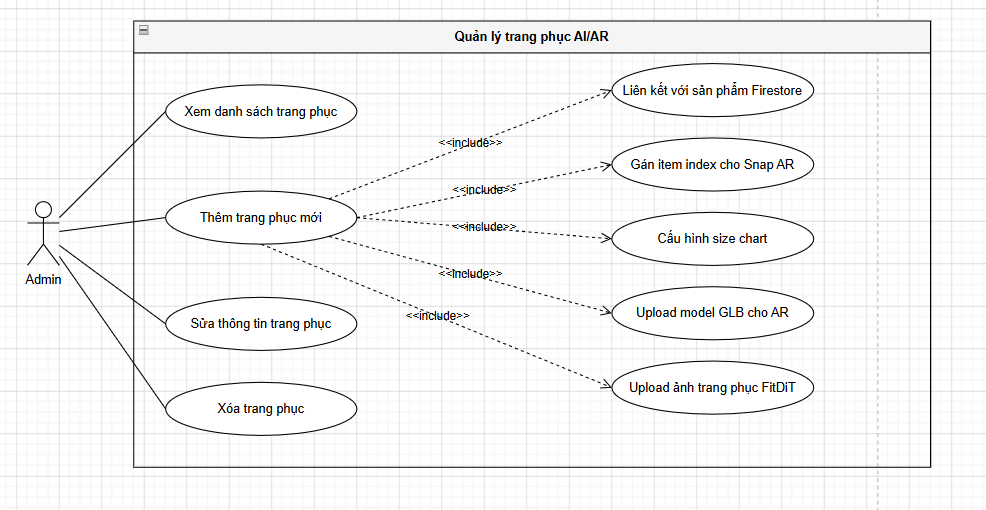
\includegraphics[width=0.8\textwidth]{graphics/main/chapter2/section2/uc_AR.jpg}
    \caption{Use case Diagram chức năng admin quản lý trang phục AI/AR}
    \label{fig:usecase_AR}
\end{figure}

\subsubsection{Đặc tả use case chức năng admin quản lý trang phục AI/AR}

\begin{longtable}{|>{\raggedright\arraybackslash}p{2cm}|>{\raggedright\arraybackslash}p{2.5cm}|>{\raggedright\arraybackslash}p{4cm}|>{\raggedright\arraybackslash}p{5.5cm}|}
\caption{Đặc tả use case chức năng admin quản lý trang phục AI/AR}
\label{tab:uc_admin_ar} \\
\hline
\rowcolor{header}\textcolor{white}{\textbf{Mã UC}} & \textcolor{white}{\textbf{Tên}} & \textcolor{white}{\textbf{Luồng chính}} & \textcolor{white}{\textbf{Ngoại lệ / Thay thế}} \\
\hline
\endfirsthead
\caption[]{Đặc tả use case chức năng admin quản lý trang phục AI/AR (tiếp theo)} \\
\hline
\rowcolor{header}\textcolor{white}{\textbf{Mã UC}} & \textcolor{white}{\textbf{Tên}} & \textcolor{white}{\textbf{Luồng chính}} & \textcolor{white}{\textbf{Ngoại lệ / Thay thế}} \\
\hline
\endhead

UC1 & Xem danh sách trang phục &
  \textbf{Tiền ĐK:} Đã đăng nhập. \newline
  1. Admin truy cập trang quản lý trang phục AI/AR. \newline
  2. Hệ thống hiển thị danh sách trang phục (tên, ảnh FitDiT, trạng thái model GLB, sản phẩm liên kết). \newline
  3. Admin lọc hoặc tìm kiếm theo tên. &
  Không có trang phục $\to$ hiển thị danh sách trống. \\
\hline

UC2 & Thêm trang phục mới &
  \textbf{Tiền ĐK:} Đã đăng nhập. \newline
  1. Admin nhập tên trang phục. \newline
  2. \textit{[include]} UC5: Upload ảnh FitDiT. \newline
  3. \textit{[include]} UC6: Upload model GLB cho AR. \newline
  4. \textit{[include]} UC7: Cấu hình size chart. \newline
  5. \textit{[include]} UC8: Gán item index Snap AR. \newline
  6. \textit{[include]} UC9: Liên kết sản phẩm Firestore. \newline
  7. Hệ thống xác thực và lưu vào CSDL. \newline
  \textbf{Hậu ĐK:} Trang phục mới được tạo đầy đủ. &
  Thiếu trường bắt buộc $\to$ lỗi validation. \newline
  Lỗi upload file $\to$ thông báo lỗi, cho phép thử lại. \\
\hline

UC3 & Sửa thông tin trang phục &
  \textbf{Tiền ĐK:} Đã đăng nhập; trang phục tồn tại. \newline
  1. Admin chọn trang phục cần sửa. \newline
  2. Hệ thống hiển thị thông tin hiện tại. \newline
  3. Admin chỉnh sửa các trường cần thay đổi. \newline
  4. Hệ thống xác thực và lưu thay đổi. &
  Lỗi lưu dữ liệu $\to$ không thay đổi, thông báo lỗi. \\
\hline

UC4 & Xóa trang phục &
  \textbf{Tiền ĐK:} Đã đăng nhập; trang phục tồn tại. \newline
  1. Admin chọn trang phục cần xóa. \newline
  2. Hệ thống hiển thị hộp thoại xác nhận. \newline
  3. Admin xác nhận $\to$ hệ thống xóa trang phục và các tài nguyên liên quan. \newline
  \textbf{Hậu ĐK:} Trang phục bị xóa khỏi CSDL. &
  Admin hủy $\to$ không thay đổi. \\
\hline

UC5 & Upload ảnh trang phục FitDiT &
  \textbf{Tiền ĐK:} Đang thực hiện UC2 hoặc UC3. \newline
  1. Admin chọn file ảnh trang phục (nền trắng, full body). \newline
  2. Hệ thống kiểm tra định dạng và kích thước. \newline
  3. Hệ thống upload lên Cloudinary và lưu URL vào CSDL. \newline
  \textbf{Hậu ĐK:} URL ảnh FitDiT được lưu. &
  Sai định dạng $\to$ thông báo lỗi. \newline
  Vượt kích thước giới hạn $\to$ yêu cầu chọn lại. \\
\hline

UC6 & Upload model GLB cho AR &
  \textbf{Tiền ĐK:} Đang thực hiện UC2 hoặc UC3. \newline
  1. Admin chọn file \texttt{.glb} của trang phục. \newline
  2. Hệ thống kiểm tra định dạng file. \newline
  3. Hệ thống lưu file vào static server FastAPI và cập nhật đường dẫn. \newline
  \textbf{Hậu ĐK:} Model GLB khả dụng qua static URL. &
  Sai định dạng (không phải \texttt{.glb}) $\to$ thông báo lỗi. \newline
  File quá lớn $\to$ yêu cầu tối ưu và upload lại. \\
\hline

UC7 & Cấu hình size chart &
  \textbf{Tiền ĐK:} Đang thực hiện UC2 hoặc UC3. \newline
  1. Admin nhập bảng kích thước (S/M/L/XL: số đo ngực, eo, hông, chiều cao). \newline
  2. Hệ thống lưu size chart vào CSDL. \newline
  \textbf{Hậu ĐK:} Size chart được liên kết với trang phục. &
  Thiếu thông số kích thước $\to$ cảnh báo trước khi lưu. \\
\hline

UC8 & Gán item index cho Snap AR &
  \textbf{Tiền ĐK:} Đang thực hiện UC2 hoặc UC3; Lens Studio đã cấu hình. \newline
  1. Admin nhập item index tương ứng với trang phục trong Lens Studio. \newline
  2. Hệ thống lưu item index vào CSDL. \newline
  \textbf{Hậu ĐK:} Item index được liên kết, Snap AR có thể nhận diện đúng trang phục. &
  Item index đã được gán cho trang phục khác $\to$ cảnh báo trùng lặp. \\
\hline

UC9 & Liên kết với sản phẩm Firestore &
  \textbf{Tiền ĐK:} Đang thực hiện UC2 hoặc UC3; sản phẩm tồn tại trên Firestore. \newline
  1. Admin chọn sản phẩm tương ứng từ danh sách Firestore. \newline
  2. Hệ thống lưu product ID liên kết vào CSDL. \newline
  \textbf{Hậu ĐK:} Trang phục được liên kết với sản phẩm để điều hướng mua hàng. &
  Sản phẩm không tồn tại trên Firestore $\to$ thông báo lỗi. \\
\hline

\end{longtable}

% ================================================================
\subsection{Use case Diagram chức năng admin quản lý cửa hàng và đánh giá}
\begin{figure}[H]
    \centering
    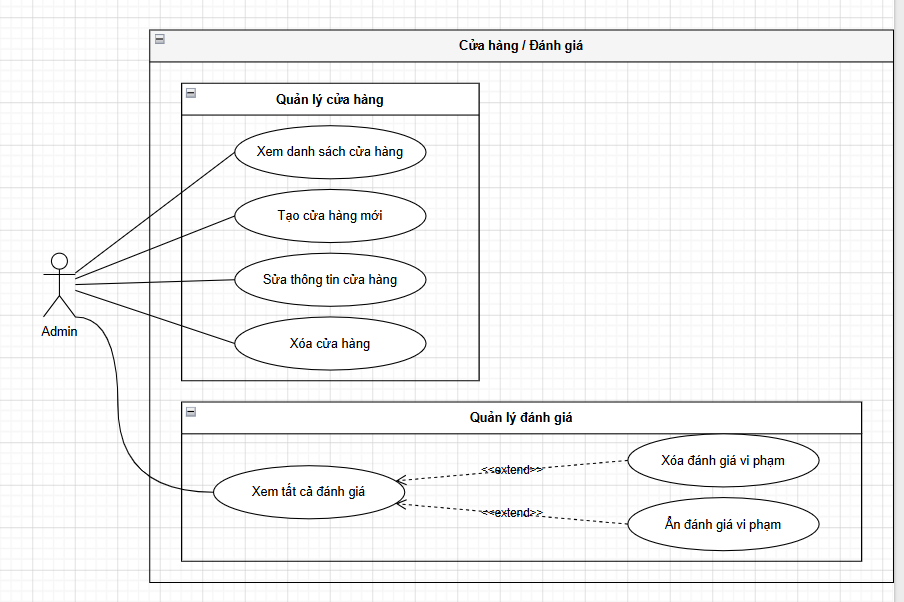
\includegraphics[width=0.8\textwidth]{graphics/main/chapter2/section2/uc_store_danhgia.jpg}
    \caption{Use case Diagram chức năng admin quản lý cửa hàng và đánh giá}
    \label{fig:usecase_store_danhgia}
\end{figure}

\subsubsection{Đặc tả use case chức năng admin quản lý cửa hàng và đánh giá}

\begin{longtable}{|>{\raggedright\arraybackslash}p{2cm}|>{\raggedright\arraybackslash}p{2.5cm}|>{\raggedright\arraybackslash}p{4cm}|>{\raggedright\arraybackslash}p{5.5cm}|}
\caption{Đặc tả use case chức năng admin quản lý cửa hàng và đánh giá}
\label{tab:uc_admin_store_review} \\
\hline
\rowcolor{header}\textcolor{white}{\textbf{Mã UC}} & \textcolor{white}{\textbf{Tên}} & \textcolor{white}{\textbf{Luồng chính}} & \textcolor{white}{\textbf{Ngoại lệ / Thay thế}} \\
\hline
\endfirsthead
\caption[]{Đặc tả use case chức năng admin quản lý cửa hàng và đánh giá (tiếp theo)} \\
\hline
\rowcolor{header}\textcolor{white}{\textbf{Mã UC}} & \textcolor{white}{\textbf{Tên}} & \textcolor{white}{\textbf{Luồng chính}} & \textcolor{white}{\textbf{Ngoại lệ / Thay thế}} \\
\hline
\endhead

\multicolumn{4}{|l|}{\cellcolor{gray!20}\textit{\textbf{Quản lý cửa hàng}}} \\
\hline

UC1 & Xem danh sách cửa hàng &
  \textbf{Tiền ĐK:} Đã đăng nhập. \newline
  1. Admin truy cập trang quản lý cửa hàng. \newline
  2. Hệ thống hiển thị danh sách cửa hàng (tên, địa chỉ, SĐT, email, trạng thái). &
  Chưa có cửa hàng $\to$ hiển thị danh sách trống. \\
\hline

UC2 & Tạo cửa hàng mới &
  \textbf{Tiền ĐK:} Đã đăng nhập. \newline
  1. Admin nhập tên, SĐT, email, địa chỉ và chấm vị trí trên bản đồ. \newline
  2. Hệ thống lấy tọa độ GPS và xác thực dữ liệu. \newline
  3. Hệ thống lưu cửa hàng vào CSDL. \newline
  \textbf{Hậu ĐK:} Cửa hàng mới được tạo. &
  Thiếu trường bắt buộc $\to$ lỗi validation. \newline
  Địa chỉ không xác định được tọa độ $\to$ yêu cầu chấm lại trên bản đồ. \\
\hline

UC3 & Sửa thông tin cửa hàng &
  \textbf{Tiền ĐK:} Đã đăng nhập; cửa hàng tồn tại. \newline
  1. Admin chọn cửa hàng cần sửa. \newline
  2. Hệ thống hiển thị thông tin hiện tại. \newline
  3. Admin chỉnh sửa các trường cần thay đổi. \newline
  4. Hệ thống xác thực và lưu thay đổi. &
  Sai định dạng email/SĐT $\to$ lỗi validation. \newline
  Lỗi lưu dữ liệu $\to$ không thay đổi, thông báo lỗi. \\
\hline

UC4 & Xóa cửa hàng &
  \textbf{Tiền ĐK:} Đã đăng nhập; cửa hàng tồn tại. \newline
  1. Admin chọn cửa hàng cần xóa. \newline
  2. Hệ thống hiển thị hộp thoại xác nhận. \newline
  3. Admin xác nhận $\to$ hệ thống xóa cửa hàng và dữ liệu liên quan. \newline
  \textbf{Hậu ĐK:} Cửa hàng bị xóa khỏi CSDL. &
  Admin hủy $\to$ không thay đổi. \\
\hline

\multicolumn{4}{|l|}{\cellcolor{gray!20}\textit{\textbf{Quản lý đánh giá}}} \\
\hline

UC5 & Xem tất cả đánh giá &
  \textbf{Tiền ĐK:} Đã đăng nhập. \newline
  1. Admin truy cập trang quản lý đánh giá. \newline
  2. Hệ thống hiển thị danh sách đánh giá (khách hàng, sản phẩm, số sao, nội dung, trạng thái). \newline
  3. Admin lọc theo sản phẩm, số sao hoặc trạng thái. \newline
  4. \textit{[extend]} UC6/UC7: Xử lý đánh giá vi phạm nếu cần. &
  Không có đánh giá $\to$ hiển thị danh sách trống. \\
\hline

UC6 & Ẩn đánh giá vi phạm &
  \textbf{Tiền ĐK:} Đang xem UC5; đánh giá đang hiển thị. \newline
  1. Admin chọn đánh giá vi phạm và chọn \textit{Ẩn}. \newline
  2. Hệ thống cập nhật trạng thái thành \textit{đã ẩn}. \newline
  \textbf{Hậu ĐK:} Đánh giá không còn hiển thị với người dùng nhưng vẫn lưu trong CSDL. &
  Admin hủy $\to$ không thay đổi. \\
\hline

UC7 & Xóa đánh giá vi phạm &
  \textbf{Tiền ĐK:} Đang xem UC5; đánh giá tồn tại. \newline
  1. Admin chọn đánh giá vi phạm và chọn \textit{Xóa}. \newline
  2. Hệ thống hiển thị hộp thoại xác nhận. \newline
  3. Admin xác nhận $\to$ hệ thống xóa vĩnh viễn khỏi CSDL. \newline
  \textbf{Hậu ĐK:} Đánh giá bị xóa hoàn toàn. &
  Admin hủy $\to$ không thay đổi. \newline
  Lỗi xóa dữ liệu $\to$ thông báo lỗi. \\
\hline

\end{longtable}

% ================================================================
\subsection{Use case Diagram chức năng người dùng mua sản phẩm}
\begin{figure}[H]
    \centering
    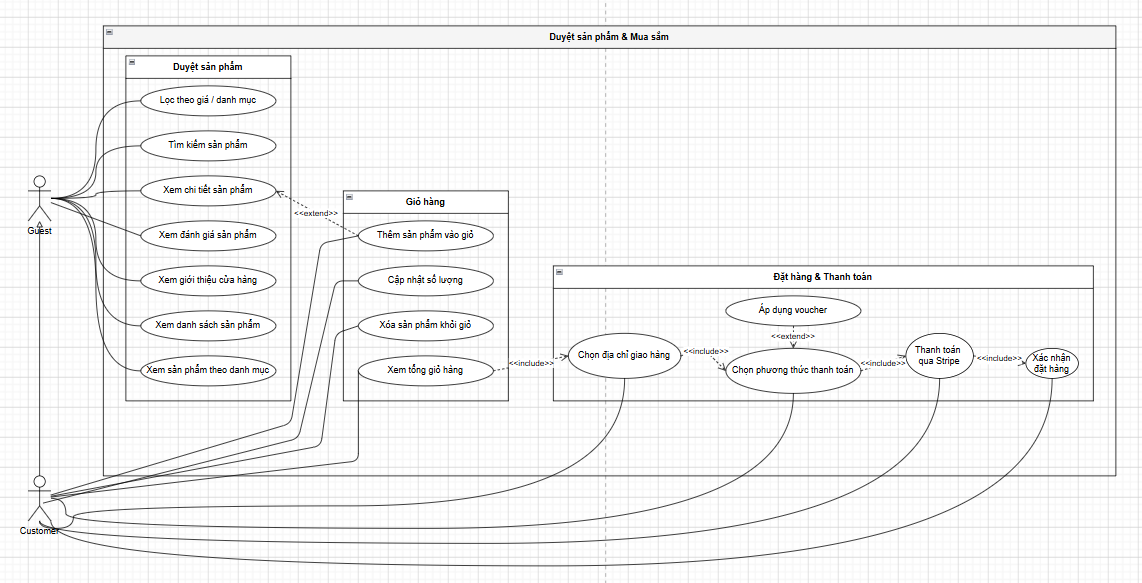
\includegraphics[width=0.8\textwidth]{graphics/main/chapter2/section2/uc_duyet_sp.jpg}
    \caption{Use case Diagram chức năng người dùng mua sản phẩm}
    \label{fig:usecase_duyet_sp}
\end{figure}

\subsubsection{Đặc tả use case chức năng duyệt sản phẩm và mua sắm}

\begin{longtable}{|>{\raggedright\arraybackslash}p{2cm}|>{\raggedright\arraybackslash}p{2.5cm}|>{\raggedright\arraybackslash}p{4cm}|>{\raggedright\arraybackslash}p{5.5cm}|}
\caption{Đặc tả use case chức năng duyệt sản phẩm và mua sắm}
\label{tab:uc_customer_shopping} \\
\hline
\rowcolor{header}\textcolor{white}{\textbf{Mã UC}} & \textcolor{white}{\textbf{Tên}} & \textcolor{white}{\textbf{Luồng chính}} & \textcolor{white}{\textbf{Ngoại lệ / Thay thế}} \\
\hline
\endfirsthead
\caption[]{Đặc tả use case chức năng duyệt sản phẩm và mua sắm (tiếp theo)} \\
\hline
\rowcolor{header}\textcolor{white}{\textbf{Mã UC}} & \textcolor{white}{\textbf{Tên}} & \textcolor{white}{\textbf{Luồng chính}} & \textcolor{white}{\textbf{Ngoại lệ / Thay thế}} \\
\hline
\endhead

\multicolumn{4}{|l|}{\cellcolor{gray!20}\textit{\textbf{Duyệt sản phẩm --- Actor: Guest}}} \\
\hline

UC1 & Xem giới thiệu cửa hàng &
  1. Guest truy cập trang giới thiệu. \newline
  2. Hệ thống hiển thị tên, địa chỉ, SĐT, email và vị trí bản đồ. &
  Lỗi tải dữ liệu $\to$ thông báo lỗi. \\
\hline

UC2 & Xem danh sách sản phẩm &
  1. Guest truy cập trang sản phẩm. \newline
  2. Hệ thống hiển thị danh sách sản phẩm (ảnh, tên, giá, đánh giá). &
  Không có sản phẩm $\to$ hiển thị thông báo trống. \\
\hline

UC3 & Xem sản phẩm theo danh mục &
  1. Guest chọn danh mục. \newline
  2. Hệ thống lọc và hiển thị sản phẩm thuộc danh mục đó. &
  Danh mục không có sản phẩm $\to$ hiển thị thông báo trống. \\
\hline

UC4 & Lọc theo giá / danh mục &
  1. Guest chọn tiêu chí lọc (khoảng giá, danh mục). \newline
  2. Hệ thống cập nhật danh sách theo tiêu chí đã chọn. &
  Không có sản phẩm phù hợp $\to$ hiển thị thông báo trống. \\
\hline

UC5 & Tìm kiếm sản phẩm &
  1. Guest nhập từ khóa vào ô tìm kiếm. \newline
  2. Hệ thống trả về danh sách sản phẩm phù hợp. &
  Không tìm thấy $\to$ hiển thị thông báo không có kết quả. \\
\hline

UC6 & Xem chi tiết sản phẩm &
  1. Guest chọn sản phẩm từ danh sách. \newline
  2. Hệ thống hiển thị: ảnh, mô tả, giá, biến thể (size/màu), tồn kho. \newline
  3. \textit{[extend]} UC8: Thêm vào giỏ nếu Guest là Customer. &
  Sản phẩm không tồn tại $\to$ thông báo lỗi, quay về danh sách. \\
\hline

UC7 & Xem đánh giá sản phẩm &
  1. Guest xem phần đánh giá trên trang chi tiết sản phẩm. \newline
  2. Hệ thống hiển thị danh sách đánh giá (số sao, nội dung, ảnh, tên người đánh giá). &
  Chưa có đánh giá $\to$ hiển thị thông báo chưa có đánh giá. \\
\hline

\multicolumn{4}{|l|}{\cellcolor{gray!20}\textit{\textbf{Giỏ hàng --- Actor: Customer}}} \\
\hline

UC8 & Thêm sản phẩm vào giỏ &
  \textbf{Tiền ĐK:} Đã đăng nhập. \newline
  1. Customer chọn biến thể (size, màu) và số lượng. \newline
  2. Hệ thống kiểm tra tồn kho và thêm vào giỏ. \newline
  \textbf{Hậu ĐK:} Sản phẩm được lưu trong giỏ hàng. &
  Sản phẩm hết hàng $\to$ thông báo, không cho thêm. \newline
  Chưa đăng nhập $\to$ chuyển hướng trang đăng nhập. \\
\hline

UC9 & Cập nhật số lượng &
  \textbf{Tiền ĐK:} Đã đăng nhập; có sản phẩm trong giỏ. \newline
  1. Customer thay đổi số lượng sản phẩm trong giỏ. \newline
  2. Hệ thống kiểm tra tồn kho và cập nhật tổng tiền. &
  Số lượng vượt tồn kho $\to$ giới hạn về số tối đa có thể đặt. \newline
  Số lượng về 0 $\to$ xóa sản phẩm khỏi giỏ. \\
\hline

UC10 & Xóa sản phẩm khỏi giỏ &
  \textbf{Tiền ĐK:} Đã đăng nhập; có sản phẩm trong giỏ. \newline
  1. Customer chọn xóa sản phẩm. \newline
  2. Hệ thống xóa và cập nhật lại tổng tiền. &
  Không có. \\
\hline

UC11 & Xem tổng giỏ hàng &
  \textbf{Tiền ĐK:} Đã đăng nhập. \newline
  1. Customer truy cập trang giỏ hàng. \newline
  2. Hệ thống hiển thị danh sách sản phẩm, số lượng, đơn giá và tổng tiền. \newline
  3. \textit{[include]} UC12: Chuyển sang đặt hàng. &
  Giỏ hàng trống $\to$ thông báo và gợi ý tiếp tục mua sắm. \\
\hline

\multicolumn{4}{|l|}{\cellcolor{gray!20}\textit{\textbf{Đặt hàng \& Thanh toán --- Actor: Customer}}} \\
\hline

UC12 & Chọn địa chỉ giao hàng &
  \textbf{Tiền ĐK:} Đang thực hiện UC11. \newline
  1. Hệ thống hiển thị danh sách địa chỉ đã lưu. \newline
  2. Customer chọn địa chỉ hoặc nhập địa chỉ mới. \newline
  3. \textit{[include]} UC13: Chuyển sang chọn phương thức thanh toán. &
  Chưa có địa chỉ $\to$ bắt buộc nhập mới trước khi tiếp tục. \\
\hline

UC13 & Chọn phương thức thanh toán &
  \textbf{Tiền ĐK:} Đang thực hiện UC12. \newline
  1. Hệ thống hiển thị các phương thức: COD, Stripe. \newline
  2. Customer chọn phương thức. \newline
  3. \textit{[extend]} UC14: Áp dụng voucher nếu có. \newline
  4. \textit{[include]} UC15: Xử lý thanh toán. &
  Không có. \\
\hline

UC14 & Áp dụng voucher &
  \textbf{Tiền ĐK:} Đang thực hiện UC13. \newline
  1. Customer nhập mã voucher. \newline
  2. Hệ thống kiểm tra điều kiện áp dụng. \newline
  3. Hệ thống tính lại tổng tiền sau giảm giá. &
  Mã không hợp lệ / hết hạn $\to$ thông báo lỗi. \newline
  Đơn hàng không đủ điều kiện $\to$ thông báo điều kiện áp dụng. \\
\hline

UC15 & Thanh toán qua Stripe &
  \textbf{Tiền ĐK:} Đang thực hiện UC13; Customer chọn Stripe. \newline
  1. Hệ thống tạo phiên thanh toán Stripe và chuyển hướng. \newline
  2. Customer nhập thông tin thẻ và xác nhận. \newline
  3. Stripe xử lý và trả kết quả về hệ thống. \newline
  4. \textit{[include]} UC16: Xác nhận đặt hàng nếu thành công. &
  Thanh toán thất bại $\to$ thông báo lỗi, đề xuất thử lại hoặc đổi phương thức. \\
\hline

UC16 & Xác nhận đặt hàng &
  \textbf{Tiền ĐK:} UC15 hoàn tất (Stripe) hoặc Customer xác nhận COD. \newline
  1. Hệ thống tạo đơn hàng, trừ tồn kho và gửi email xác nhận. \newline
  2. Hệ thống hiển thị trang thành công kèm mã đơn hàng. \newline
  \textbf{Hậu ĐK:} Đơn hàng được tạo với trạng thái \textit{chờ xác nhận}. &
  Lỗi tạo đơn $\to$ thông báo lỗi, không trừ tồn kho. \\
\hline

\end{longtable}

% ================================================================
\subsection{Use case Diagram chức năng người dùng quản lý đơn hàng, địa chỉ và đánh giá}
\begin{figure}[H]
    \centering
    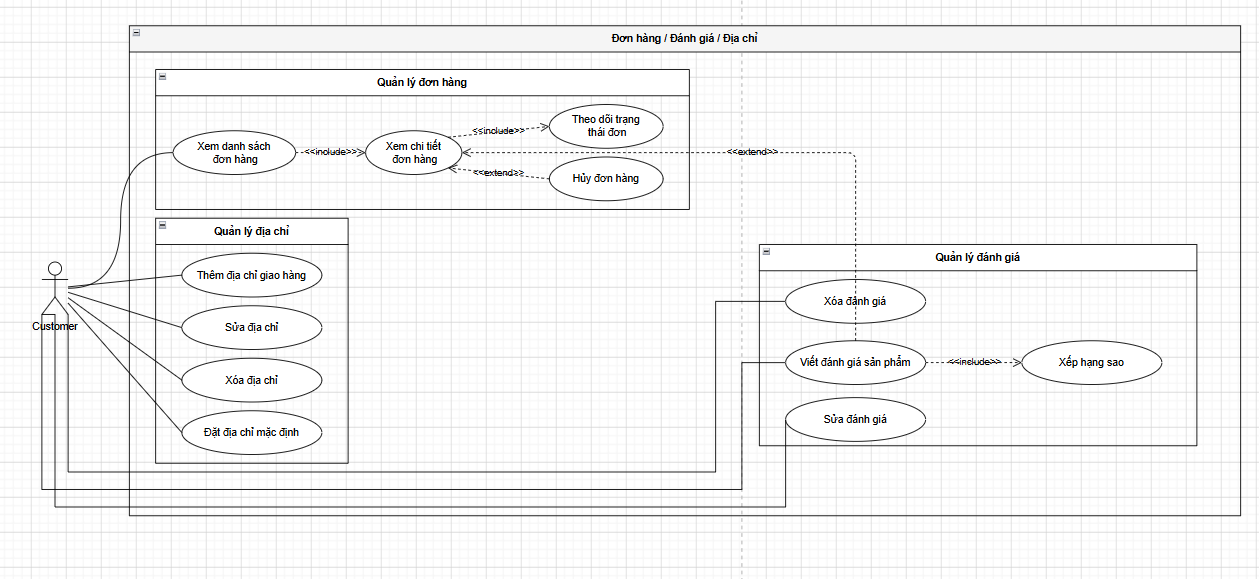
\includegraphics[width=0.8\textwidth]{graphics/main/chapter2/section2/uc_dia_chi.jpg}
    \caption{Use case Diagram chức năng người dùng quản lý đơn hàng, địa chỉ và đánh giá}
    \label{fig:usecase_diachi}
\end{figure}

\subsubsection{Đặc tả use case chức năng quản lý đơn hàng, đánh giá và địa chỉ}

\begin{longtable}{|>{\raggedright\arraybackslash}p{2cm}|>{\raggedright\arraybackslash}p{2.5cm}|>{\raggedright\arraybackslash}p{4cm}|>{\raggedright\arraybackslash}p{5.5cm}|}
\caption{Đặc tả use case chức năng quản lý đơn hàng, đánh giá và địa chỉ}
\label{tab:uc_customer_order_review_address} \\
\hline
\rowcolor{header}\textcolor{white}{\textbf{Mã UC}} & \textcolor{white}{\textbf{Tên}} & \textcolor{white}{\textbf{Luồng chính}} & \textcolor{white}{\textbf{Ngoại lệ / Thay thế}} \\
\hline
\endfirsthead
\caption[]{Đặc tả use case chức năng quản lý đơn hàng, đánh giá và địa chỉ (tiếp theo)} \\
\hline
\rowcolor{header}\textcolor{white}{\textbf{Mã UC}} & \textcolor{white}{\textbf{Tên}} & \textcolor{white}{\textbf{Luồng chính}} & \textcolor{white}{\textbf{Ngoại lệ / Thay thế}} \\
\hline
\endhead

\multicolumn{4}{|l|}{\cellcolor{gray!20}\textit{\textbf{Quản lý đơn hàng --- Actor: Customer}}} \\
\hline

UC1 & Xem danh sách đơn hàng &
  \textbf{Tiền ĐK:} Đã đăng nhập. \newline
  1. Customer truy cập mục \textit{Đơn hàng của tôi}. \newline
  2. Hệ thống hiển thị danh sách đơn (mã đơn, ngày đặt, trạng thái, tổng tiền). \newline
  3. \textit{[include]} UC2: Xem chi tiết khi chọn đơn. &
  Chưa có đơn hàng $\to$ hiển thị thông báo trống. \\
\hline

UC2 & Xem chi tiết đơn hàng &
  \textbf{Tiền ĐK:} Đã chọn đơn từ UC1. \newline
  1. Hệ thống hiển thị: sản phẩm, địa chỉ giao, phương thức thanh toán, tổng tiền. \newline
  2. \textit{[include]} UC3: Hiển thị trạng thái hiện tại. \newline
  3. \textit{[extend]} UC4: Hiển thị nút hủy nếu đơn cho phép. &
  Đơn không tồn tại $\to$ thông báo lỗi, quay về danh sách. \\
\hline

UC3 & Theo dõi trạng thái đơn &
  \textbf{Tiền ĐK:} Đang xem UC2. \newline
  1. Hệ thống hiển thị timeline trạng thái: chờ xác nhận $\to$ đã xác nhận $\to$ đang giao $\to$ đã giao. \newline
  2. \textit{[extend]} UC5: Hiển thị nút đánh giá khi đơn đã giao. &
  Không có. \\
\hline

UC4 & Hủy đơn hàng &
  \textbf{Tiền ĐK:} Đơn ở trạng thái \textit{chờ xác nhận}. \newline
  1. Customer chọn \textit{Hủy đơn} và nhập lý do. \newline
  2. Hệ thống xác nhận lại hành động. \newline
  3. Customer xác nhận $\to$ hệ thống gửi yêu cầu hủy đến Admin. \newline
  \textbf{Hậu ĐK:} Yêu cầu hủy được ghi nhận, chờ Admin xử lý. &
  Đơn đã xác nhận/đang giao $\to$ không cho phép hủy, thông báo liên hệ hỗ trợ. \\
\hline

\multicolumn{4}{|l|}{\cellcolor{gray!20}\textit{\textbf{Quản lý đánh giá --- Actor: Customer}}} \\
\hline

UC5 & Viết đánh giá sản phẩm &
  \textbf{Tiền ĐK:} Đơn hàng ở trạng thái \textit{đã giao hàng}. \newline
  1. Customer chọn sản phẩm cần đánh giá từ đơn đã hoàn tất. \newline
  2. Customer nhập nội dung nhận xét và tùy chọn đính kèm ảnh. \newline
  3. \textit{[include]} UC6: Xếp hạng sao. \newline
  4. Customer gửi $\to$ hệ thống lưu và hiển thị đánh giá. \newline
  \textbf{Hậu ĐK:} Đánh giá được lưu và hiển thị tại trang sản phẩm. &
  Đơn chưa hoàn tất $\to$ không cho phép đánh giá. \newline
  Đã đánh giá sản phẩm này $\to$ chuyển sang UC7. \\
\hline

UC6 & Xếp hạng sao &
  \textbf{Tiền ĐK:} Đang thực hiện UC5. \newline
  1. Customer chọn số sao từ 1 đến 5. \newline
  2. Hệ thống ghi nhận số sao vào đánh giá. &
  Chưa chọn sao $\to$ cảnh báo bắt buộc trước khi gửi. \\
\hline

UC7 & Sửa đánh giá &
  \textbf{Tiền ĐK:} Đã đăng nhập; đánh giá do chính Customer tạo. \newline
  1. Customer chọn \textit{Sửa đánh giá}. \newline
  2. Hệ thống hiển thị nội dung hiện tại. \newline
  3. Customer chỉnh sửa nội dung/số sao/ảnh và lưu. \newline
  \textbf{Hậu ĐK:} Đánh giá được cập nhật. &
  Lỗi lưu dữ liệu $\to$ thông báo lỗi, không thay đổi. \\
\hline

UC8 & Xóa đánh giá &
  \textbf{Tiền ĐK:} Đã đăng nhập; đánh giá do chính Customer tạo. \newline
  1. Customer chọn \textit{Xóa đánh giá}. \newline
  2. Hệ thống xác nhận lại hành động. \newline
  3. Customer xác nhận $\to$ hệ thống xóa đánh giá. \newline
  \textbf{Hậu ĐK:} Đánh giá bị xóa khỏi trang sản phẩm. &
  Customer hủy $\to$ không thay đổi. \\
\hline

\multicolumn{4}{|l|}{\cellcolor{gray!20}\textit{\textbf{Quản lý địa chỉ --- Actor: Customer}}} \\
\hline

UC9 & Thêm địa chỉ giao hàng &
  \textbf{Tiền ĐK:} Đã đăng nhập. \newline
  1. Customer nhập họ tên, SĐT, địa chỉ chi tiết (tỉnh/thành, quận/huyện, phường/xã). \newline
  2. Hệ thống xác thực và lưu địa chỉ. \newline
  \textbf{Hậu ĐK:} Địa chỉ mới được thêm vào danh sách. &
  Thiếu trường bắt buộc $\to$ lỗi validation. \\
\hline

UC10 & Sửa địa chỉ &
  \textbf{Tiền ĐK:} Đã đăng nhập; địa chỉ tồn tại. \newline
  1. Customer chọn địa chỉ cần sửa. \newline
  2. Hệ thống hiển thị thông tin hiện tại. \newline
  3. Customer chỉnh sửa và lưu. &
  Thiếu trường bắt buộc $\to$ lỗi validation. \\
\hline

UC11 & Xóa địa chỉ &
  \textbf{Tiền ĐK:} Đã đăng nhập; địa chỉ tồn tại. \newline
  1. Customer chọn \textit{Xóa} địa chỉ. \newline
  2. Hệ thống xác nhận $\to$ xóa khỏi danh sách. &
  Địa chỉ đang là mặc định $\to$ yêu cầu đặt địa chỉ mặc định khác trước. \\
\hline

UC12 & Đặt địa chỉ mặc định &
  \textbf{Tiền ĐK:} Đã đăng nhập; có ít nhất một địa chỉ. \newline
  1. Customer chọn địa chỉ muốn đặt làm mặc định. \newline
  2. Hệ thống cập nhật địa chỉ mặc định và bỏ mặc định của địa chỉ cũ. \newline
  \textbf{Hậu ĐK:} Địa chỉ được đánh dấu mặc định, tự động chọn khi đặt hàng. &
  Không có. \\
\hline

\end{longtable}

% ================================================================
\subsection{Use case Diagram chức năng người dùng sử dụng FitDit-AI}
\begin{figure}[H]
    \centering
    \includegraphics[width=0.8\textwidth]{graphics/main/chapter2/section2/uc_photo_AR.jpg}
    \caption{Use case Diagram chức năng người dùng sử dụng FitDit-AI}
    \label{fig:usecase_photo_AR}
\end{figure}

\subsubsection{Đặc tả use case chức năng FitDiT AI -- Photo Try-On}

\begin{longtable}{|>{\raggedright\arraybackslash}p{2cm}|>{\raggedright\arraybackslash}p{2.5cm}|>{\raggedright\arraybackslash}p{4cm}|>{\raggedright\arraybackslash}p{5.5cm}|}
\caption{Đặc tả use case chức năng FitDiT AI -- Photo Try-On}
\label{tab:uc_fitdit_ai} \\
\hline
\rowcolor{header}\textcolor{white}{\textbf{Mã UC}} & \textcolor{white}{\textbf{Tên}} & \textcolor{white}{\textbf{Luồng chính}} & \textcolor{white}{\textbf{Ngoại lệ / Thay thế}} \\
\hline
\endfirsthead
\caption[]{Đặc tả use case chức năng FitDiT AI -- Photo Try-On (tiếp theo)} \\
\hline
\rowcolor{header}\textcolor{white}{\textbf{Mã UC}} & \textcolor{white}{\textbf{Tên}} & \textcolor{white}{\textbf{Luồng chính}} & \textcolor{white}{\textbf{Ngoại lệ / Thay thế}} \\
\hline
\endhead

UC1 & Upload ảnh người dùng &
  \textbf{Tiền ĐK:} Đã đăng nhập. \newline
  1. Customer chọn hoặc chụp ảnh toàn thân. \newline
  2. Hệ thống kiểm tra định dạng và chất lượng ảnh. \newline
  3. \textit{[include]} UC4: Kích hoạt pipeline AI sau khi đủ đầu vào. \newline
  \textbf{Hậu ĐK:} Ảnh người dùng sẵn sàng cho bước generate. &
  Sai định dạng $\to$ thông báo lỗi. \newline
  Không phát hiện người trong ảnh $\to$ yêu cầu upload lại ảnh rõ hơn. \\
\hline

UC2 & Chọn trang phục để thử &
  \textbf{Tiền ĐK:} Đã đăng nhập. \newline
  1. Customer duyệt danh sách trang phục AI/AR và chọn một trang phục. \newline
  2. \textit{[include]} UC4: Kích hoạt pipeline AI sau khi đủ đầu vào. &
  Chưa có trang phục nào $\to$ thông báo danh sách trống. \\
\hline

UC3 & Chọn loại: áo / quần / tổng thể &
  \textbf{Tiền ĐK:} Đã chọn trang phục (UC2). \newline
  1. Customer chọn loại thử: áo, quần hoặc tổng thể. \newline
  2. \textit{[include]} UC4: Truyền tham số loại vào pipeline AI. &
  Không có. \\
\hline

UC4 & Chạy AI generate ảnh &
  \textbf{Tiền ĐK:} UC1, UC2, UC3 đã hoàn tất. \newline
  1. Hệ thống gửi ảnh người dùng, ảnh trang phục và loại thử đến FitDiT API. \newline
  2. FitDiT xử lý và trả về ảnh kết quả. \newline
  3. \textit{[include]} UC5: Hiển thị kết quả. \newline
  \textbf{Hậu ĐK:} Ảnh thử đồ ảo được tạo thành công. &
  API timeout $\to$ thông báo lỗi, cho phép thử lại. \newline
  Chất lượng đầu vào thấp $\to$ FitDiT trả lỗi, yêu cầu upload ảnh tốt hơn. \\
\hline

UC5 & Xem kết quả thử đồ ảo &
  \textbf{Tiền ĐK:} UC4 hoàn tất thành công. \newline
  1. Hệ thống hiển thị ảnh kết quả thử đồ. \newline
  2. \textit{[extend]} UC6: Lưu ảnh nếu Customer muốn. \newline
  3. \textit{[extend]} UC8: Xem lịch sử nếu Customer muốn. &
  Không có. \\
\hline

UC6 & Lưu ảnh kết quả &
  \textbf{Tiền ĐK:} Đang xem kết quả UC5. \newline
  1. Customer chọn \textit{Lưu ảnh}. \newline
  2. Hệ thống upload ảnh lên Cloudinary và lưu URL vào lịch sử thử đồ của Customer. \newline
  3. \textit{[extend]} UC7: Tải ảnh về máy nếu Customer muốn. \newline
  \textbf{Hậu ĐK:} Ảnh được lưu vào lịch sử và Cloudinary. &
  Lỗi upload $\to$ thông báo lỗi, cho phép thử lại. \\
\hline

UC7 & Tải ảnh kết quả về máy &
  \textbf{Tiền ĐK:} Đang xem UC6 hoặc UC5. \newline
  1. Customer chọn \textit{Tải về}. \newline
  2. Hệ thống tạo link download và trả file ảnh về thiết bị. \newline
  \textbf{Hậu ĐK:} Ảnh được lưu vào bộ nhớ thiết bị. &
  Lỗi tải file $\to$ thông báo lỗi. \\
\hline

UC8 & Xem lịch sử thử đồ &
  \textbf{Tiền ĐK:} Đã đăng nhập. \newline
  1. Customer truy cập mục lịch sử thử đồ. \newline
  2. Hệ thống hiển thị danh sách ảnh kết quả đã lưu (ảnh, trang phục, ngày thử). \newline
  3. \textit{[extend]} UC9: Xóa lịch sử nếu Customer muốn. &
  Chưa có lịch sử $\to$ hiển thị thông báo trống. \\
\hline

UC9 & Xóa lịch sử thử đồ &
  \textbf{Tiền ĐK:} Đang xem UC8; có ít nhất một bản ghi lịch sử. \newline
  1. Customer chọn ảnh cần xóa hoặc chọn \textit{Xóa tất cả}. \newline
  2. Hệ thống xác nhận lại hành động. \newline
  3. Customer xác nhận $\to$ hệ thống xóa bản ghi và ảnh trên Cloudinary. \newline
  \textbf{Hậu ĐK:} Lịch sử được xóa khỏi hệ thống. &
  Customer hủy $\to$ không thay đổi. \newline
  Lỗi xóa $\to$ thông báo lỗi. \\
\hline

\end{longtable}

% ================================================================
\subsection{Use case Diagram chức năng người dùng sử dụng snap camera}
\begin{figure}[H]
    \centering
    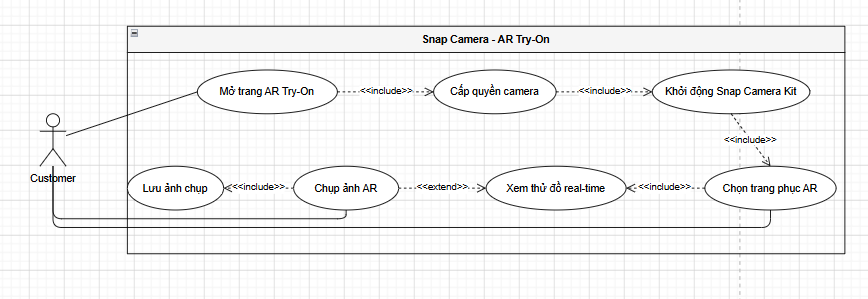
\includegraphics[width=0.8\textwidth]{graphics/main/chapter2/section2/uc_snap.jpg}
    \caption{Use case Diagram chức năng người dùng sử dụng snap camera}
    \label{fig:usecase_snap_camera}
\end{figure}

\subsubsection{Đặc tả use case chức năng Snap Camera -- AR Try-On}

\begin{longtable}{|>{\raggedright\arraybackslash}p{2cm}|>{\raggedright\arraybackslash}p{2.5cm}|>{\raggedright\arraybackslash}p{4cm}|>{\raggedright\arraybackslash}p{5.5cm}|}
\caption{Đặc tả use case chức năng Snap Camera -- AR Try-On}
\label{tab:uc_snap_ar} \\
\hline
\rowcolor{header}\textcolor{white}{\textbf{Mã UC}} & \textcolor{white}{\textbf{Tên}} & \textcolor{white}{\textbf{Luồng chính}} & \textcolor{white}{\textbf{Ngoại lệ / Thay thế}} \\
\hline
\endfirsthead
\caption[]{Đặc tả use case chức năng Snap Camera -- AR Try-On (tiếp theo)} \\
\hline
\rowcolor{header}\textcolor{white}{\textbf{Mã UC}} & \textcolor{white}{\textbf{Tên}} & \textcolor{white}{\textbf{Luồng chính}} & \textcolor{white}{\textbf{Ngoại lệ / Thay thế}} \\
\hline
\endhead

UC1 & Mở trang AR Try-On &
  \textbf{Tiền ĐK:} Đã đăng nhập. \newline
  1. Customer truy cập trang AR Try-On. \newline
  2. \textit{[include]} UC2: Yêu cầu cấp quyền camera. &
  Trình duyệt không hỗ trợ WebGL/Camera Kit $\to$ thông báo yêu cầu đổi trình duyệt. \\
\hline

UC2 & Cấp quyền camera &
  \textbf{Tiền ĐK:} Đang thực hiện UC1. \newline
  1. Hệ thống hiển thị hộp thoại xin quyền camera. \newline
  2. Customer chấp nhận. \newline
  3. \textit{[include]} UC3: Khởi động Snap Camera Kit. \newline
  \textbf{Hậu ĐK:} Luồng camera được kích hoạt. &
  Customer từ chối $\to$ thông báo cần cấp quyền để sử dụng tính năng, dừng luồng. \\
\hline

UC3 & Khởi động Snap Camera Kit &
  \textbf{Tiền ĐK:} Quyền camera đã được cấp (UC2). \newline
  1. Hệ thống khởi tạo Snap Camera Kit SDK. \newline
  2. SDK tải lens mặc định và render lên canvas. \newline
  3. \textit{[include]} UC4: Hiển thị danh sách trang phục AR để chọn. \newline
  \textbf{Hậu ĐK:} Camera Kit sẵn sàng, luồng video hiển thị trên giao diện. &
  Lỗi tải SDK $\to$ thông báo lỗi, yêu cầu tải lại trang. \newline
  Lỗi tải lens $\to$ thông báo lỗi kết nối Snap. \\
\hline

UC4 & Chọn trang phục AR &
  \textbf{Tiền ĐK:} Camera Kit đã khởi động (UC3). \newline
  1. Hệ thống hiển thị danh sách trang phục AR có sẵn. \newline
  2. Customer chọn một trang phục. \newline
  3. Hệ thống gửi item index tương ứng đến Snap Lens Studio. \newline
  4. \textit{[include]} UC5: Hiển thị thử đồ real-time. &
  Danh sách trang phục trống $\to$ thông báo chưa có trang phục AR. \newline
  Lỗi tải model GLB $\to$ thông báo lỗi, cho phép chọn trang phục khác. \\
\hline

UC5 & Xem thử đồ real-time &
  \textbf{Tiền ĐK:} Đã chọn trang phục (UC4). \newline
  1. Snap Lens render model 3D GLB lên body tracking của Customer theo thời gian thực. \newline
  2. Customer di chuyển để xem trang phục từ nhiều góc độ. \newline
  3. \textit{[extend]} UC6: Chụp ảnh nếu Customer muốn lưu kết quả. &
  Mất body tracking $\to$ model tạm thời ẩn, tự phục hồi khi phát hiện lại. \newline
  Ánh sáng yếu $\to$ chất lượng tracking giảm, hiển thị cảnh báo. \\
\hline

UC6 & Chụp ảnh AR &
  \textbf{Tiền ĐK:} Đang xem thử đồ real-time (UC5). \newline
  1. Customer nhấn nút chụp. \newline
  2. Hệ thống capture frame hiện tại từ canvas Camera Kit. \newline
  3. \textit{[include]} UC7: Lưu ảnh chụp. \newline
  \textbf{Hậu ĐK:} Ảnh AR được tạo và lưu thành công. &
  Lỗi capture canvas $\to$ thông báo lỗi, cho phép thử lại. \\
\hline

UC7 & Lưu ảnh chụp &
  \textbf{Tiền ĐK:} Ảnh AR đã được capture (UC6). \newline
  1. Hệ thống upload ảnh lên Cloudinary. \newline
  2. Hệ thống lưu URL vào lịch sử của Customer. \newline
  3. Hệ thống cung cấp tùy chọn tải ảnh về thiết bị. \newline
  \textbf{Hậu ĐK:} Ảnh được lưu trên Cloudinary và hiển thị trong lịch sử. &
  Lỗi upload $\to$ thông báo lỗi, cho phép thử lại hoặc lưu cục bộ. \\
\hline

\end{longtable}

% ================================================================

\subsection{Use case Diagram chức năng người dùng gợi ý size quần áo}
\begin{figure}[H]
    \centering
    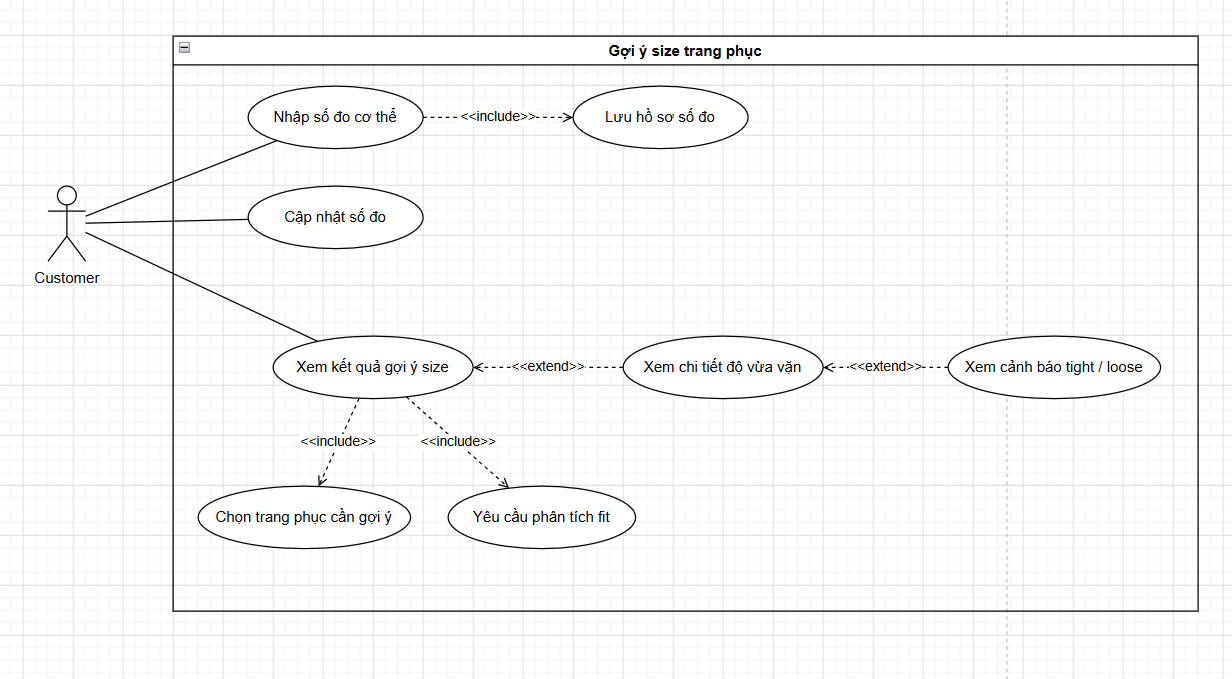
\includegraphics[width=0.8\textwidth]{graphics/main/chapter2/section2/uc_size.jpg}
    \caption{Use case Diagram chức năng người dùng gợi ý size quần áo}
    \label{fig:usecase_size}
\end{figure}

\subsubsection{Đặc tả use case chức năng gợi ý size trang phục}

\begin{longtable}{|>{\raggedright\arraybackslash}p{2cm}|>{\raggedright\arraybackslash}p{2.5cm}|>{\raggedright\arraybackslash}p{4cm}|>{\raggedright\arraybackslash}p{5.5cm}|}
\caption{Đặc tả use case chức năng gợi ý size trang phục}
\label{tab:usecase_size_2} \\
\hline
\rowcolor{header}\textcolor{white}{\textbf{Mã UC}} & \textcolor{white}{\textbf{Tên}} & \textcolor{white}{\textbf{Luồng chính}} & \textcolor{white}{\textbf{Ngoại lệ / Thay thế}} \\
\hline
\endfirsthead

\multicolumn{4}{c}{\tablename\ \thetable{} -- \textit{(tiếp theo)}} \\
\hline
\rowcolor{header}\textcolor{white}{\textbf{Mã UC}} & \textcolor{white}{\textbf{Tên}} & \textcolor{white}{\textbf{Luồng chính}} & \textcolor{white}{\textbf{Ngoại lệ / Thay thế}} \\
\hline
\endhead

\hline
\multicolumn{4}{r}{\textit{Chuyển trang tiếp theo...}} \\
\endfoot

\hline
\endlastfoot

UC1 & Nhập số đo cơ thể &
  \textbf{Tiền ĐK:} Đã đăng nhập. \newline
  1. Customer nhập các số đo: chiều cao, cân nặng, vòng ngực, vòng eo, vòng hông. \newline
  2. Hệ thống xác thực dữ liệu đầu vào. \newline
  3. \textit{[include]} UC2: Lưu hồ sơ số đo. &
  Thiếu trường bắt buộc $\to$ lỗi validation. \newline
  Giá trị ngoài khoảng hợp lệ $\to$ cảnh báo và yêu cầu nhập lại. \\
\hline

UC2 & Lưu hồ sơ số đo &
  \textbf{Tiền ĐK:} Đang thực hiện UC1; dữ liệu hợp lệ. \newline
  1. Hệ thống lưu hồ sơ số đo vào CSDL liên kết với tài khoản Customer. \newline
  \textbf{Hậu ĐK:} Hồ sơ số đo được lưu, sẵn sàng dùng cho gợi ý size. &
  Lỗi lưu CSDL $\to$ thông báo lỗi, cho phép thử lại. \\
\hline

UC3 & Cập nhật số đo &
  \textbf{Tiền ĐK:} Đã đăng nhập; hồ sơ số đo đã tồn tại. \newline
  1. Customer truy cập trang hồ sơ số đo. \newline
  2. Hệ thống hiển thị số đo hiện tại. \newline
  3. Customer chỉnh sửa các trường cần thay đổi và lưu. \newline
  \textbf{Hậu ĐK:} Hồ sơ số đo được cập nhật. &
  Giá trị không hợp lệ $\to$ lỗi validation. \\
\hline

UC4 & Chọn trang phục cần gợi ý &
  \textbf{Tiền ĐK:} Đã đăng nhập; hồ sơ số đo đã lưu. \newline
  1. Customer duyệt danh sách trang phục và chọn một trang phục muốn biết size phù hợp. \newline
  2. \textit{[include]} UC5: Yêu cầu phân tích fit. &
  Chưa có hồ sơ số đo $\to$ chuyển hướng sang UC1. \newline
  Trang phục không có size chart $\to$ thông báo chưa hỗ trợ gợi ý size. \\
\hline

UC5 & Yêu cầu phân tích fit &
  \textbf{Tiền ĐK:} Đang thực hiện UC4. \newline
  1. Hệ thống lấy số đo từ hồ sơ Customer và size chart của trang phục. \newline
  2. Hệ thống so sánh số đo với từng mức size (S/M/L/XL). \newline
  3. \textit{[include]} UC6: Trả về kết quả gợi ý. \newline
  \textbf{Hậu ĐK:} Phân tích độ vừa vặn hoàn tất. &
  Size chart không đủ thông số $\to$ thông báo không thể phân tích đầy đủ. \\
\hline

UC6 & Xem kết quả gợi ý size &
  \textbf{Tiền ĐK:} UC5 hoàn tất. \newline
  1. Hệ thống hiển thị size được gợi ý (ví dụ: \textit{Nên chọn size M}). \newline
  2. \textit{[include]} UC7: Xem chi tiết độ vừa vặn từng số đo. &
  Không có size phù hợp $\to$ hiển thị size gần nhất kèm lưu ý. \\
\hline

UC7 & Xem chi tiết độ vừa vặn &
  \textbf{Tiền ĐK:} Đang xem UC6. \newline
  1. Hệ thống hiển thị bảng so sánh chi tiết từng số đo của Customer với size được gợi ý (ngực, eo, hông, chiều cao). \newline
  2. \textit{[extend]} UC8: Hiển thị cảnh báo nếu có số đo tight/loose. &
  Không có. \\
\hline

UC8 & Xem cảnh báo tight / loose &
  \textbf{Tiền ĐK:} Đang xem UC7; có ít nhất một số đo vượt ngưỡng cho phép. \newline
  1. Hệ thống xác định số đo quá chật (\textit{tight}) hoặc quá rộng (\textit{loose}) so với size gợi ý. \newline
  2. Hệ thống hiển thị cảnh báo cụ thể (ví dụ: \textit{Vòng ngực hơi chật, cân nhắc size L}). \newline
  \textbf{Hậu ĐK:} Customer nhận được tư vấn chi tiết để quyết định size phù hợp nhất. &
  Tất cả số đo đều trong ngưỡng $\to$ UC8 không được kích hoạt. \\
\hline

\end{longtable}
% ================================================================
\subsection{Use case Diagram chức năng người dùng sử dụng chat AI tư vấn}
\begin{figure}[H]
    \centering
    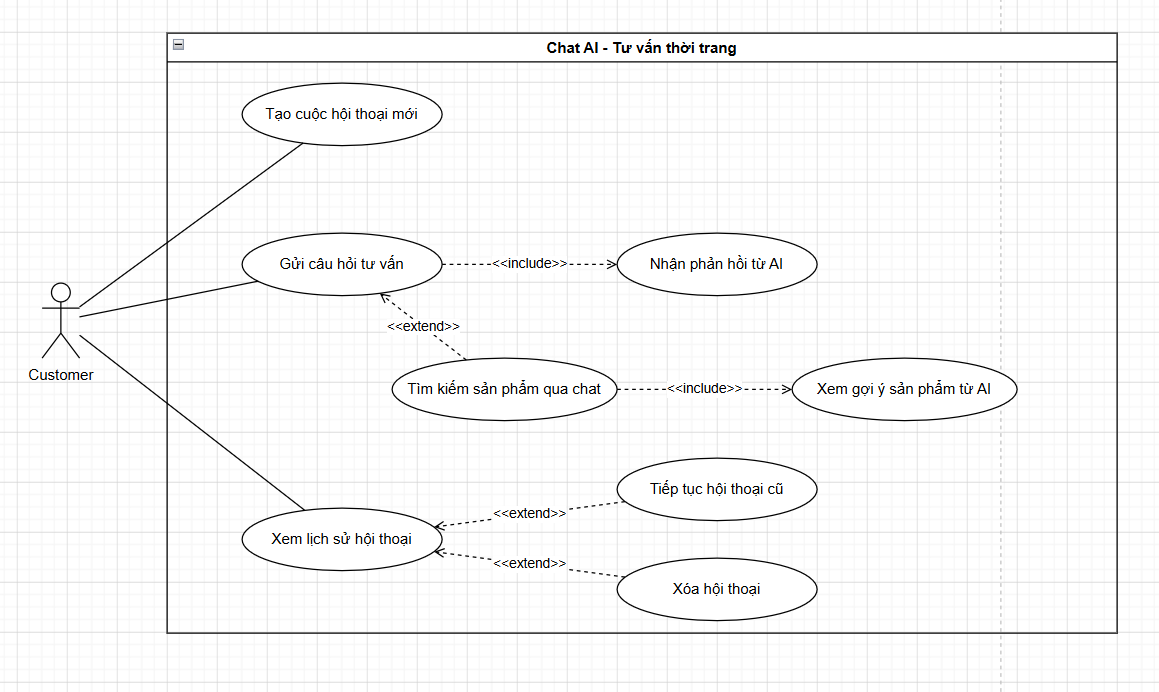
\includegraphics[width=0.8\textwidth]{graphics/main/chapter2/section2/uc_tu_van.jpg}
    \caption{Use case Diagram chức năng người dùng sử dụng chat AI tư vấn}
    \label{fig:usecase_tu_van}
\end{figure}

\subsubsection{Đặc tả use case chức năng Chat AI -- Tư vấn thời trang}

\begin{longtable}{|>{\raggedright\arraybackslash}p{2cm}|>{\raggedright\arraybackslash}p{2.5cm}|>{\raggedright\arraybackslash}p{4cm}|>{\raggedright\arraybackslash}p{5.5cm}|}
\caption{Đặc tả use case chức năng Chat AI -- Tư vấn thời trang}
\label{tab:usecase_tu_van} \\
\hline
\rowcolor{header}\textcolor{white}{\textbf{Mã UC}} & \textcolor{white}{\textbf{Tên}} & \textcolor{white}{\textbf{Luồng chính}} & \textcolor{white}{\textbf{Ngoại lệ / Thay thế}} \\
\hline
\endfirsthead

\multicolumn{4}{c}{\tablename\ \thetable{} -- \textit{(tiếp theo)}} \\
\hline
\rowcolor{header}\textcolor{white}{\textbf{Mã UC}} & \textcolor{white}{\textbf{Tên}} & \textcolor{white}{\textbf{Luồng chính}} & \textcolor{white}{\textbf{Ngoại lệ / Thay thế}} \\
\hline
\endhead

\hline
\multicolumn{4}{r}{\textit{Chuyển trang tiếp theo...}} \\
\endfoot

\hline
\endlastfoot

UC1 & Tạo cuộc hội thoại mới &
  \textbf{Tiền ĐK:} Đã đăng nhập. \newline
  1. Customer chọn \textit{Chat mới}. \newline
  2. Hệ thống tạo session hội thoại mới và hiển thị giao diện chat. \newline
  3. \textit{[include]} UC2: Customer bắt đầu gửi câu hỏi. \newline
  \textbf{Hậu ĐK:} Session hội thoại được khởi tạo trong CSDL. &
  Lỗi tạo session $\to$ thông báo lỗi, yêu cầu thử lại. \\
\hline

UC2 & Gửi câu hỏi tư vấn &
  \textbf{Tiền ĐK:} Session hội thoại đang hoạt động (UC1 hoặc UC7). \newline
  1. Customer nhập câu hỏi và gửi. \newline
  2. Hệ thống lưu tin nhắn vào lịch sử hội thoại. \newline
  3. \textit{[include]} UC3: Nhận phản hồi từ AI. &
  Câu hỏi rỗng $\to$ không cho phép gửi. \newline
  Mất kết nối $\to$ thông báo lỗi, giữ nội dung đã nhập. \\
\hline

UC3 & Nhận phản hồi từ AI &
  \textbf{Tiền ĐK:} Đang thực hiện UC2. \newline
  1. Hệ thống chuyển câu hỏi thành vector embedding. \newline
  2. Hệ thống tìm kiếm context liên quan trong vector store (pgvector). \newline
  3. Hệ thống gửi câu hỏi kèm context đến Ollama LLM. \newline
  4. AI trả về phản hồi $\to$ hệ thống hiển thị và lưu vào lịch sử. \newline
  5. \textit{[extend]} UC4: Tìm kiếm sản phẩm nếu phản hồi liên quan đến gợi ý mua hàng. &
  Không tìm thấy context $\to$ AI trả lời dựa trên kiến thức chung. \newline
  Lỗi kết nối Ollama $\to$ thông báo lỗi, yêu cầu thử lại. \newline
  Câu hỏi ngoài chủ đề $\to$ AI từ chối và hướng dẫn hỏi đúng chủ đề. \\
\hline

UC4 & Tìm kiếm sản phẩm qua chat &
  \textbf{Tiền ĐK:} AI xác định câu hỏi có liên quan đến tư vấn sản phẩm cụ thể. \newline
  1. Hệ thống trích xuất từ khóa sản phẩm từ phản hồi AI. \newline
  2. Hệ thống truy vấn CSDL sản phẩm theo từ khóa. \newline
  3. \textit{[include]} UC5: Hiển thị gợi ý sản phẩm trong luồng chat. &
  Không tìm thấy sản phẩm phù hợp $\to$ AI thông báo không có sản phẩm khớp. \\
\hline

UC5 & Xem gợi ý sản phẩm từ AI &
  \textbf{Tiền ĐK:} UC4 trả về kết quả sản phẩm. \newline
  1. Hệ thống hiển thị danh sách sản phẩm gợi ý ngay trong khung chat (ảnh, tên, giá). \newline
  2. Customer có thể nhấn vào sản phẩm để xem chi tiết. \newline
  \textbf{Hậu ĐK:} Customer được điều hướng đến trang chi tiết sản phẩm nếu chọn. &
  Sản phẩm đã hết hàng $\to$ hiển thị trạng thái hết hàng kèm gợi ý thay thế. \\
\hline

UC6 & Xem lịch sử hội thoại &
  \textbf{Tiền ĐK:} Đã đăng nhập. \newline
  1. Customer truy cập mục lịch sử chat. \newline
  2. Hệ thống hiển thị danh sách các hội thoại cũ (tiêu đề, ngày tạo, tin nhắn cuối). \newline
  3. \textit{[extend]} UC7: Tiếp tục hội thoại cũ nếu Customer chọn. \newline
  4. \textit{[extend]} UC8: Xóa hội thoại nếu Customer muốn. &
  Chưa có hội thoại nào $\to$ hiển thị thông báo trống. \\
\hline

UC7 & Tiếp tục hội thoại cũ &
  \textbf{Tiền ĐK:} Đang xem UC6; hội thoại tồn tại. \newline
  1. Customer chọn một hội thoại từ danh sách. \newline
  2. Hệ thống tải lại toàn bộ lịch sử tin nhắn của hội thoại đó. \newline
  3. Customer tiếp tục gửi câu hỏi \textit{[include UC2]}. \newline
  \textbf{Hậu ĐK:} Hội thoại được nối tiếp với context cũ. &
  Lỗi tải lịch sử $\to$ thông báo lỗi, cho phép thử lại. \\
\hline

UC8 & Xóa hội thoại &
  \textbf{Tiền ĐK:} Đang xem UC6; hội thoại tồn tại. \newline
  1. Customer chọn hội thoại cần xóa và nhấn \textit{Xóa}. \newline
  2. Hệ thống hiển thị xác nhận. \newline
  3. Customer xác nhận $\to$ hệ thống xóa hội thoại và toàn bộ tin nhắn liên quan. \newline
  \textbf{Hậu ĐK:} Hội thoại bị xóa vĩnh viễn khỏi CSDL. &
  Customer hủy $\to$ không thay đổi. \newline
  Lỗi xóa $\to$ thông báo lỗi. \\
\hline

\end{longtable}